\documentclass[oneside]{usachtesis} %%clase para tesis usach
%%package para bibliografía
\usepackage[
backend=bibtex,
sorting=none,
style=nature,
citestyle=numeric-comp
]{biblatex}



\bibliography{../bibtexs/Nanosintesis} %%bibliografía: Nanosintesis.bib
\makeindex
\setcounter{tocdepth}{1}
\graphicspath{{Imagenes/}}

\newcommand*\circled[1]{%
	\tikz[baseline=-5]{\node[draw,circle,inner sep=1pt] {#1};}
	}

%============================================================
%===================Comienzo del documento===================
%============================================================
\begin{document}
%%PORTADA						
 \title{Síntesis de Grafeno por medios químicos y construcción de supercondensadores basados en grafeno}
 \author{Carlos Eugenio}
 \facultad{CIENCIA}
 \departamento{FÍSICA}
 \profesorguia{DINESH PRATAP SINGH}
 \tituloprofesional{Ingeniero Físico}
 \anolol{2016}
 
\begin{titlepage}
	\maketitle
\end{titlepage}

\newpage
\mbox{}
\thispagestyle{empty}
\pagenumbering{roman}

%%DERECHOS DE AUTOR
\derechosdeautor

%%HOJA DE CALIFICACIONES
\newpage
\thispagestyle{empty}

%%DEDICATORIA
\newpage
\chapter*{}
\begin{flushright}
\textit{Dedicado a...}
\end{flushright}
\newpage

%%AGRADECIMIENTOS(OPTATIVA)
\chapter*{Agradecimientos}

%%TABLA DE CONTENIDOS
\newpage
\tableofcontents
\newpage
\newrgbcolor{xdxdff}{0.49 0.49 1}
\newrgbcolor{ffqqtt}{1 0 0.2}
\psset{xunit=1.0cm,yunit=1.0cm,algebraic=true,dotstyle=*,dotsize=3pt
0,linewidth=0.8pt,arrowsize=3pt 2,arrowinset=0.25}

%%ÍNDICE DE TABLAS
\newpage
\listoftables
\newrgbcolor{xdxdff}{0.49 0.49 1}
\newrgbcolor{ffqqtt}{1 0 0.2}
\psset{xunit=1.0cm,yunit=1.0cm,algebraic=true,dotstyle=*,dotsize=3pt
	0,linewidth=0.8pt,arrowsize=3pt 2,arrowinset=0.25}

%%INDICE DE ILUSTRACIONES
\newpage
\listoffigures
\newrgbcolor{xdxdff}{0.49 0.49 1}
\newrgbcolor{ffqqtt}{1 0 0.2}
\psset{xunit=1.0cm,yunit=1.0cm,algebraic=true,dotstyle=*,dotsize=3pt
0,linewidth=0.8pt,arrowsize=3pt 2,arrowinset=0.25}

%%RESUMEN
\newpage
%%RESUMEN
\chapter*{Resumen}
\addcontentsline{toc}{chapter}{Resumen}
El grafeno es un nanomaterial que encuentra su lugar en un ancho espectro de aplicaciones. En este trabajo de tesis se explora su potencial como material activo en electrodos para supercondensadores.\\
Con este objetivo, se sintetiza óxido de grafeno reducido (rGO), material cuyas propiedades físicas se acercan a las del grafeno como tal. La vía de síntesis empleada comienza con grafito natural en hojuelas, que a causa de un agente oxidante fuerte, se convierte en óxido de grafeno. En este caso, el agente oxidante utilizado es heptaóxido de manganeso (\ce{MnO_7}). Luego, éste es reducido por medio de ácido ascórbico (\ce{C_6H_8O_6}), dando como producto final óxido de grafeno reducido.\\
Este último es utilizado como material activo en la fabricación de electrodos de supercondensadores, empleando diferentes sustratos metálicos y métodos de deposición. Para caracterizar el desempeño de tales electrodos, se diseña y construye una celda de prueba, que en conjunto con la metodología de medición, resulta ser apropiada para estudiar diferencias entre los métodos de fabricación de electrodos.\\
Se concluye que el mejor desempeño se consigue utilizando óxido reducido de grafeno liofilizado y depositado en sustratos metálicos no porosos. Sin embargo, considerando el costo de este proceso, se concluye que la mejor forma de preparar electrodos, es usando láminas similares al papel fabricadas mediante filtración al vacío.\\
\hfill
\textbf{Palabras claves:} Supercondensadores, óxido reducido de grafeno, nanomateriales.

\addcontentsline{toc}{chapter}{Resumen}

%%CAPÍTULOS
\newpage
\pagenumbering{arabic}
%%%INTRODUCCIÓN GENERAL%%%
\chapter*{Introducción}
\addcontentsline{toc}{chapter}{Introducción}

El prefijo nano deriva del griego \emph{nanos}, que significa literalmente ``enano''. En el sistema internacional de unidades, el prefijo nano representa un factor de $\mathrm{10^{-9}}$, o una mil millonésima parte. Al añadir este prefijo a la unidad de longitud, obtenemos ``nanómetro'' (nm), o una mil millonésima parte de un metro. Así la nanotecnología es, a grandes rasgos, la ciencia, tecnología, e ingeniería que trata sistemas en el rango aproximado de 1-100 nanómetros. \citep{Haick2013,Gressler2013}. Se ha de tener claro en que rango de dimensiones se encuentra la escala nanométrica, los seres humanos estamos acostumbrados a escalas grandes, se nos hace fácil entender las comparaciones de kilómetros con metros, o milímetros con metros, pero al reducir el tamaño a micrómetros o nanómetros nos cuesta, pues son escalas que se escapan de nuestros sentidos. Para ponerlo en perspectiva, un nanómetro esa un metro como un metro es a un millón de kilómetros. La figura \ref{fig:scale} muestra una escala de tamaños con varios ejemplos desde la escala humana hasta la atómica, la nanoescala comprende aproximadamente desde los cientos de nanómetros hasta fracciones de nanómetros.

\begin{figure}[h!]
	\centering
	\fbox{
		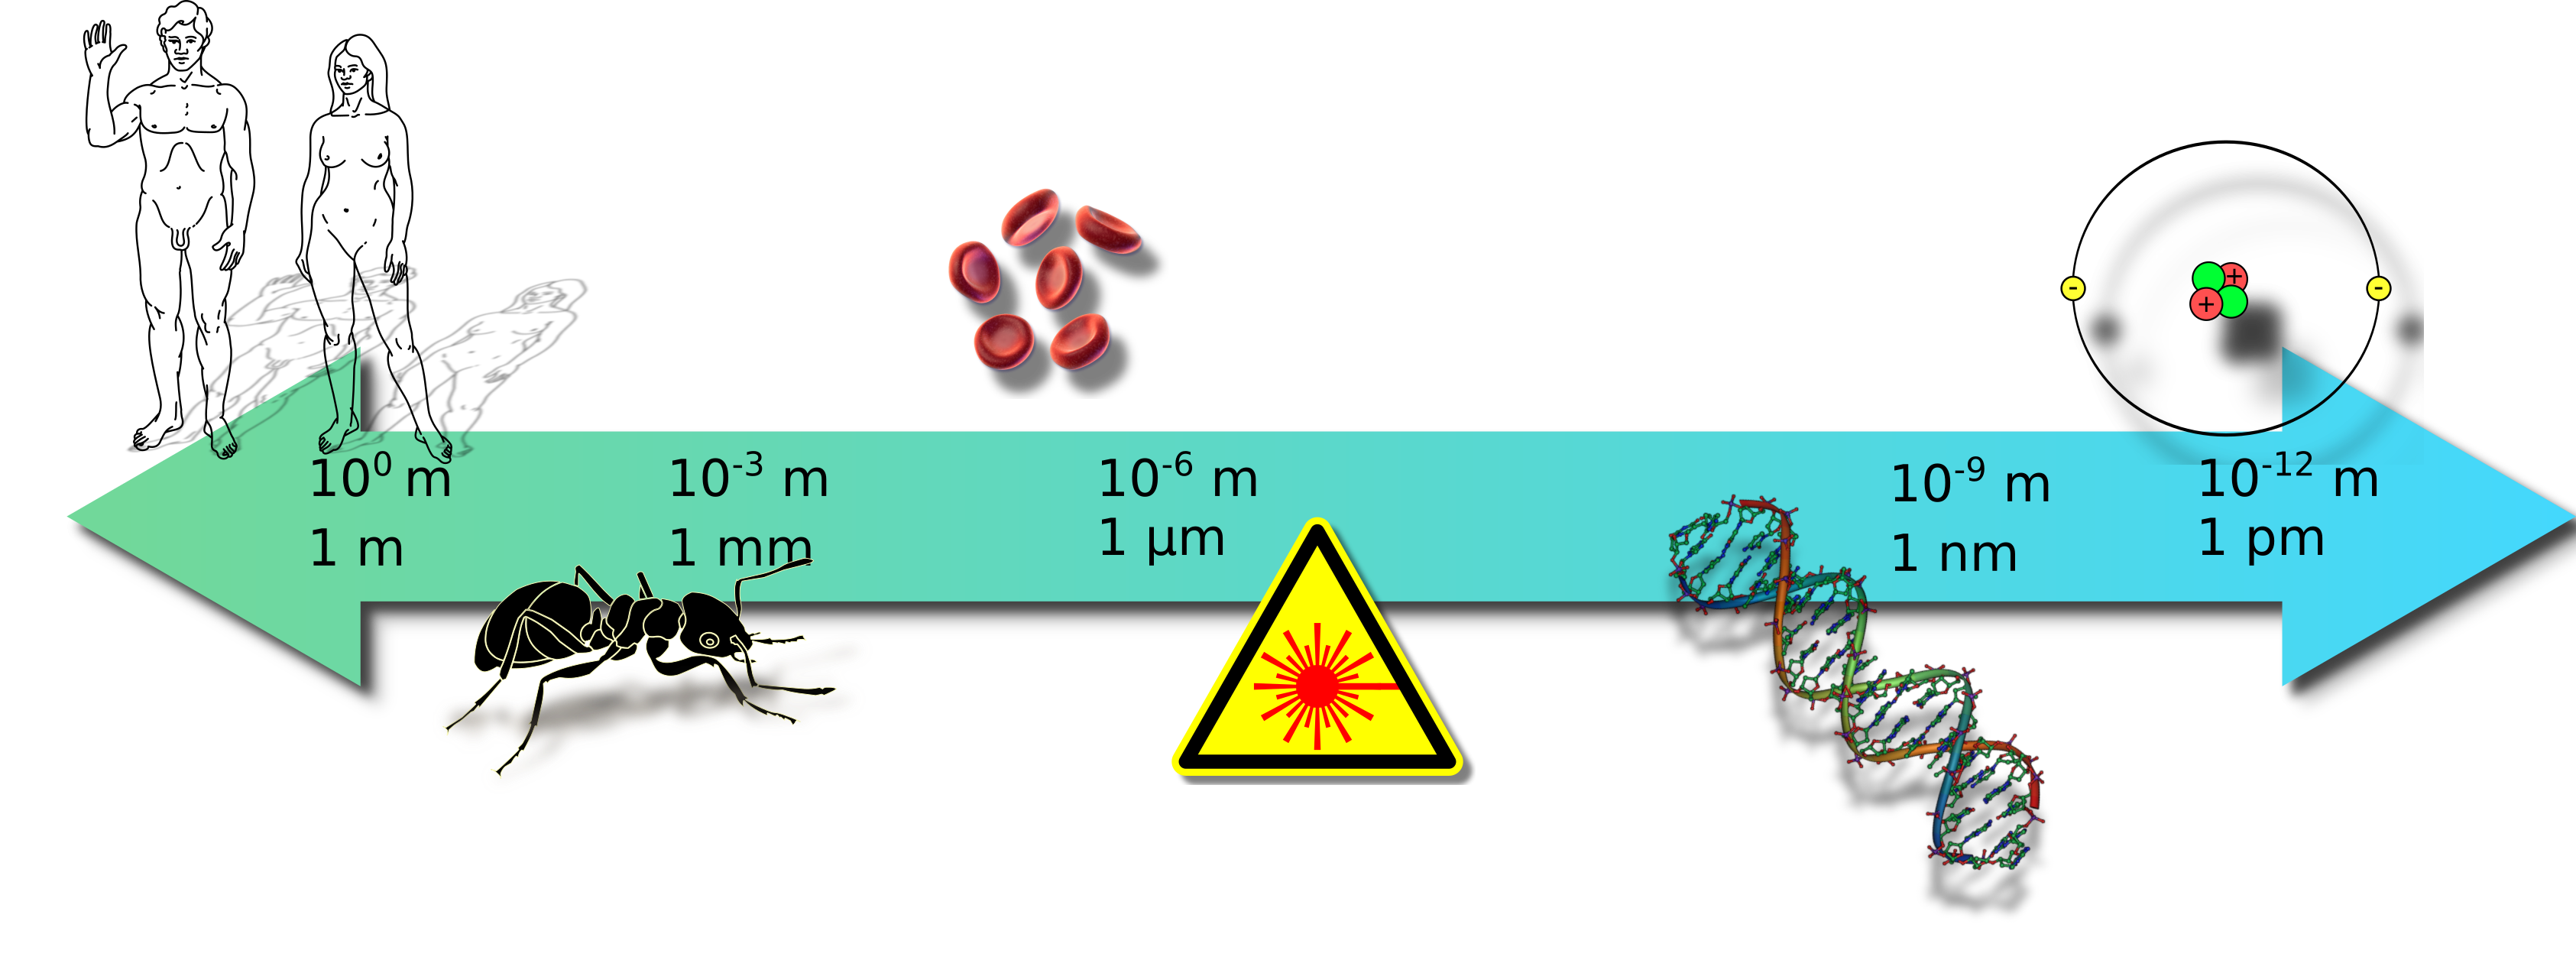
\includegraphics[width=\textwidth]{scale.png}
	}
	\caption[Comparativa de ódenes de magnitud desde metros hasta picometros]{Comparativa de órdenes de magnitud. De izquierda a derecha: Escala humana 1-2 m. Insectos 10 cm - 1 mm. Glóbulos rojos 6 $\mathrm{\mu}$m. Longitud de onda de luz visible 780-380 nm. Doble hélice de ADN 2 nm. Radio atómico de un átomo de helio 31 pm.}
\label{fig:scale}
\end{figure}

La idea de la nanotecnología fue vislumbrada por el físico Richard Feynman y expuesta en su charla \emph{``There is plenty room at the bottom''} \citep{Feynman1960}. Allí Feynman plantea que no existen barreras físicas que impidan manipular sistemas nanométricos, moléculas, o incluso átomos. La era moderna de la nanotecnología comienza con el desarrollo del microscopio de efecto túnel por Binning y Rohrer en 1981 \citep{Binnig1982}, que les hizo ganar el Premio Nobel de Física en 1986. Un microscopio de efecto túnel (STM por sus siglas en inglés \emph{Scanning Tunneling Microscope}), puede superar resoluciones de 0,1 nm de resolución lateral, y 0,01 nm en profundidad, y trabajar en variadas condiciones, sin necesidad de alto vacío o bajas temperaturas. Además de poder resolver átomos, el STM también puede manipularlos \citep{Chen2008}.

Una forma simple de clasificar los nanomateriales surge del número de dimensiones del material que no están en la nanoescala (ver figura \ref{fig:carbon_allotropes}). Un material que no posee ninguna dimensión en la nanoescala (material \emph{bulk}), se denomina material 3D y no  se considera un nanomaterial\footnote{A veces se les llama nanomateriales 3D a materiales formados por nanomateriales (2D, 1D, o 0D), que forman estructuras tridimensionales macroscópicas y muestran propiedades de nanomateriales, como por ejemplo, los aerogeles.}. Si una dimensión del material está en la nanoescala, se habla de material 2D, análogamente, con dos dimensiones en la nanoescala se trata de un nanomaterial 1D, y por último, si todas las dimensiones están en la nanoescala se denomina nanomaterial 0D.
\begin{figure}
	\centering
	\fbox{
		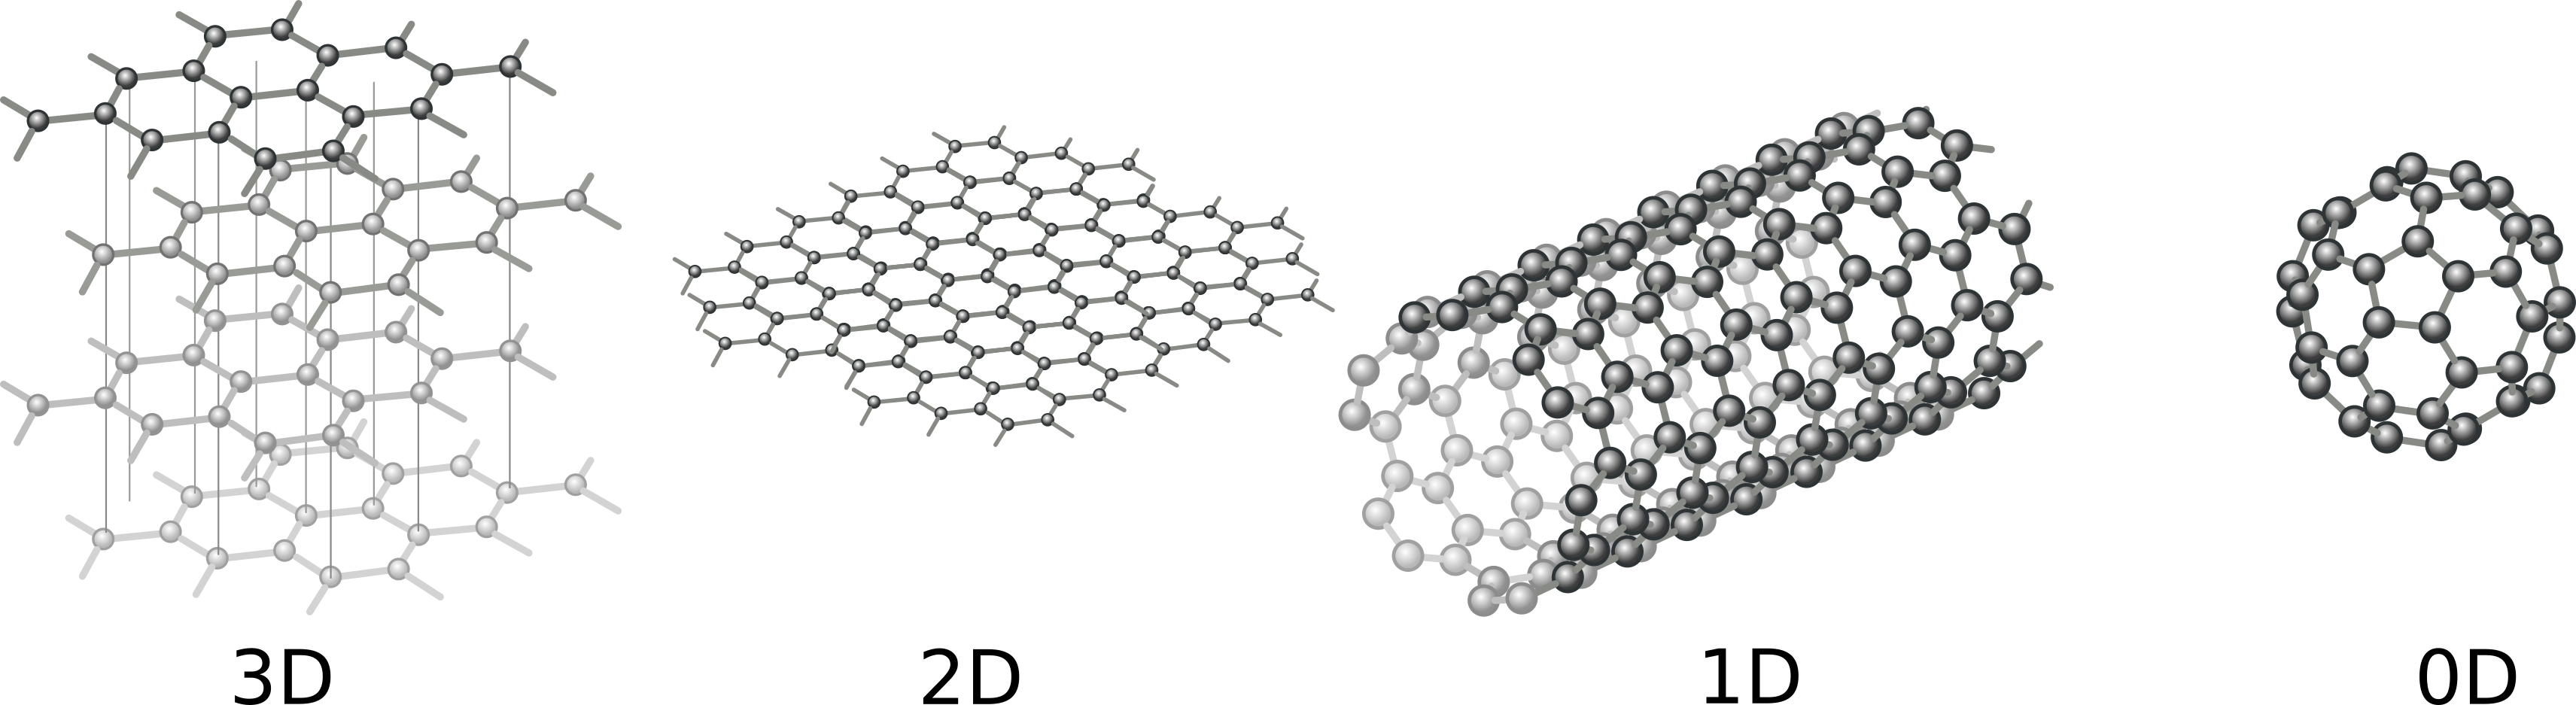
\includegraphics[width=\textwidth]{carbon_alotropes.png}
		}
	\caption[Alótropos del carbono mostrando las diferentes dimensionalidades de los nanomateriales]{Alótropos del carbono como representación de las diferentes dimensionalidades en los nanomateriales. De izquierda a derecha: Grafito, no es un material nanoestructurado, a pesar de estar formado por varios capas de grafeno. Grafeno, solo un átomo de espesor, es un material 2D. Nanotubo de carbono, es un material 1D. Fulereno, es un material 0D.}
	\label{fig:carbon_allotropes}
\end{figure}

\section*{La física de sistemas nanométricos}


%CONFINAMIENTO cuántico
Al reducir las dimensiones a escalas nanométricas, surgen efectos de confinamiento cuántico, pues se restringe el movimiento de los electrones en el material, esto conlleva a la discretización de los niveles de energía de los electrones y al cambio de la densidad de estados del material. 



%DENSIDAD de estados en diferentes dimensiones
Dependiendo de cuantas dimensiones son llevadas a la nanoescala, es como se ve afectada la densidad de estados.

\begin{figure}[h!]
	\centering
	\fbox{
		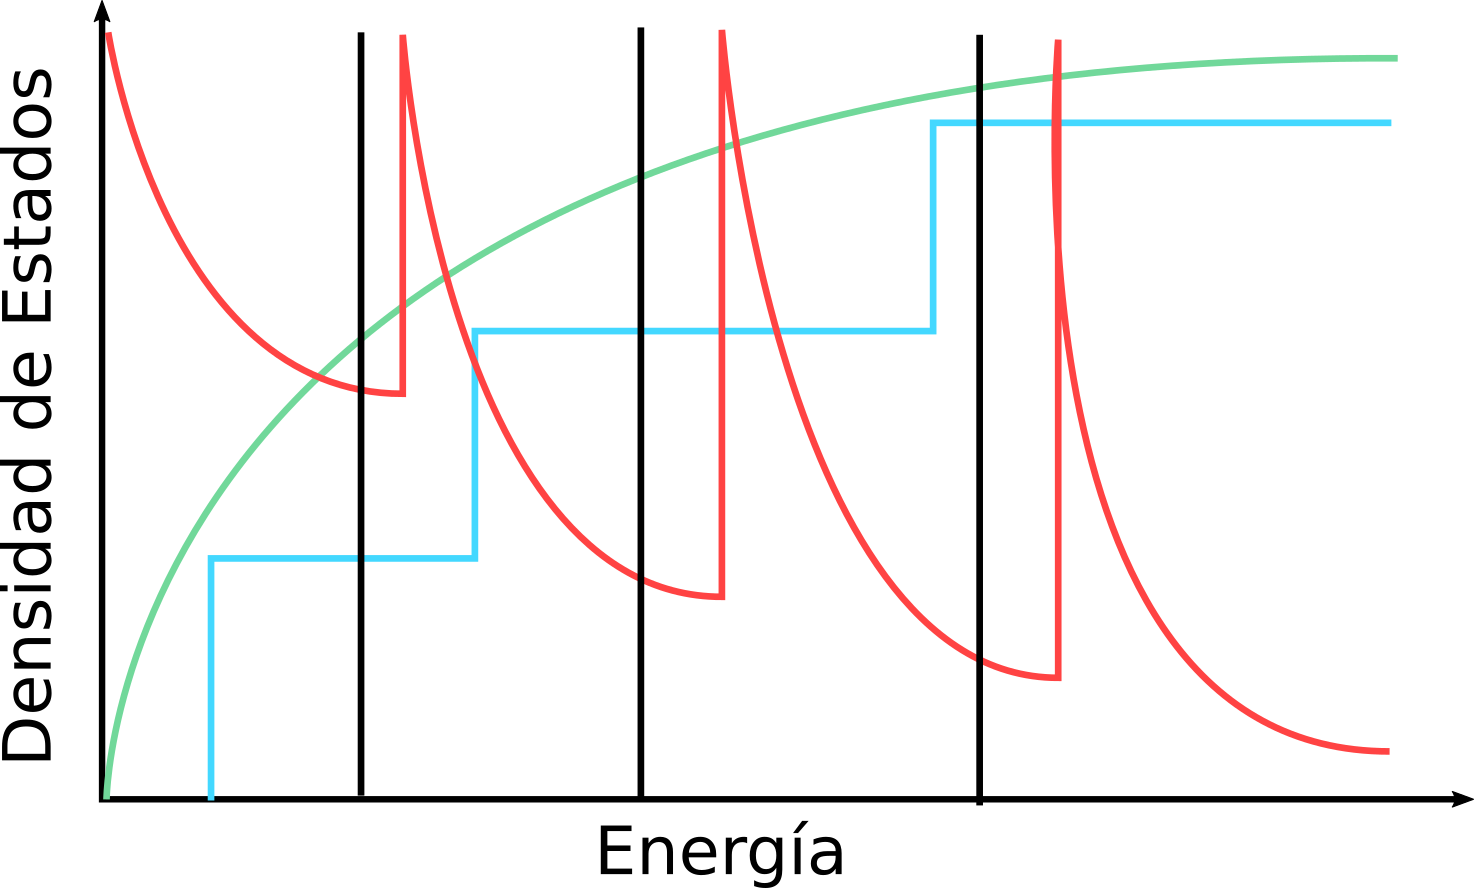
\includegraphics[width=0.6\textwidth]{DoE.png}
	}
	\caption[Densidad de estados en diferentes dimensionalidades]{Densidad de estados diferentes dimensiones. Para materiales 3D (no nanoestructurados), la densidad de estados es continua. En nanomateriales 2D, la densidad de estado forma escalones. Para materiales 1D, ésta es}
	\label{fig:DoE}
\end{figure}

%AREA superficial
Al dividir un volumen en partículas más pequeñas, el área superficial aumenta. Por ejemplo, en la secuencia de la figura \ref{fig:area_cubes}, el volumen total en cada división no cambia, pero el área superficial se dobla \footnotemark, siguiendo está lógica, al reducir un cubo de lado 1 cm a 100 nm, el área total habrá aumentado 100.000 veces. El aumento del área superficial aumenta la reactividad del material, ya que hay más lugar para, por ejemplo, reacciones químicas. Otra forma de verlo, es considerar la proporción de átomos en la superficie, con la cantidad de átomos del interior (proporción de área superficial al volumen), esta proporción aumenta al disminuir el tamaño de las partículas.

\footnotetext{Si en la secuencia de la figura \ref{fig:area_cubes} el cubo más grande tiene lado $l$, su área superficial es $6 \times l^2$, en la primera división, el lado de cada cubo es $l/2$ y el área de cada uno es $6\left( l/2\right)^2$, que en total hacen $6\left(l/2\right)^2\times 8$, en la segunda división el área total es $6\left(l/4\right)^2\times 8 \times 8$, así, en la n-ésima división el área es $6l^2 \left(1/2^n\right)^2\times 8^n$ o $6l^2 \times 2^n$. Así, el área superficial se dobla con cada división.}

\begin{figure}[h!]
	\centering
	\fbox{
		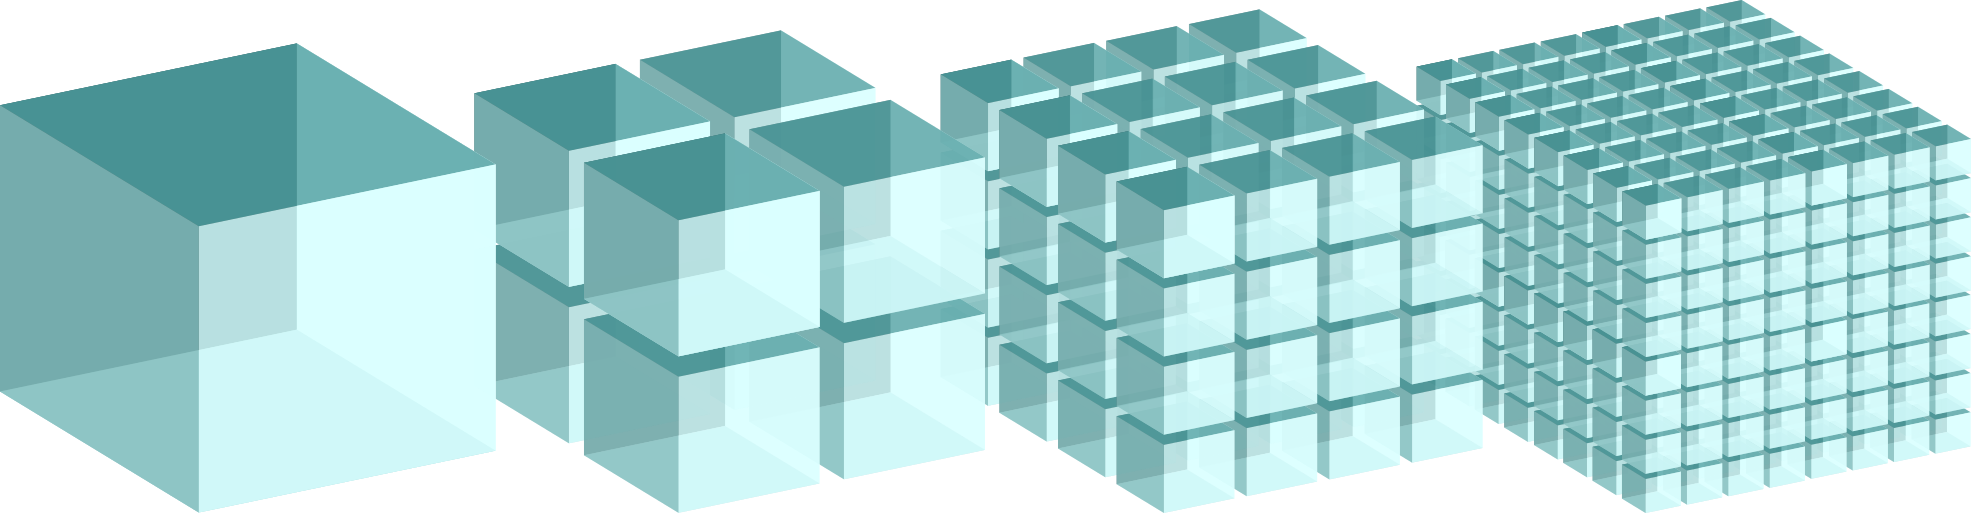
\includegraphics[width=\textwidth]{area_cubes.png}
		}
	
	\caption[Subdivisiones de un cubo demostrando el aumento de área superficial total]{Secuencia de divisiones de un cubo conservando el volumen (cantidad de material). Si se comienza con un cubo de 1 cm de lado y se subdivide hasta tener cubos de 100 nm de lado, el área superficial total pasaría de 6 $\mathrm{cm^2}$ a 60 $\mathrm{m^2}$. En este caso, el lado de un cubo disminuye 100.000 veces, aumentando el área superficial total por el mismo factor.}
	\label{fig:area_cubes}
\end{figure}

\section*{Síntesis de nanomateriales}
Dependiendo de la vía de aproximación a la nanoescala, se distinguen dos formas de síntesis, por un lado, si partimos de la forma macroscópica de un material y de algún modo se reducen sus dimensiones hacia la nanoescala, se habla de un proceso \textit{top-down}. Por ejemplo, la exfoliación del grafito (\textit{bulk material}) para obtener grafeno (nanomaterial) \citep{Novoselov2004}.  Por otro lado, sintetizar un nanomaterial a partir de átomos o moléculas es un proceso \textit{bottom-up}, un ejemplo es la síntesis de nanopartículas de oro a partir de un precursor como el ácido tetracloroaúrico \citep{Daniel2004}.

\section*{Caracterización de nanomateriales}

\part{Marco teórico}
\chapter{Nanomateriales}
	%\chapter{Nanomateriales} //is included in Marco teorico file
\noindent
\rule{\linewidth}{1 pt}
\begin{flushright}
	\begin{quotation}
		\small{
			\textit{``There’s Plenty of Room at the Bottom.''}}
	\end{quotation}
	\bf{Richard Feymann}
\end{flushright}
\noindent
\rule{\linewidth}{1 pt}\\
\vfill
\section{Nanomateriales}
%TODO ejemplos de longitudes características
Generalmente la denominación nano es atribuida a materiales en que algunas de sus dimensiones estén en la escala nanométrica, entre 1-100 nm \cite{Gressler2013}. Ésta definición es práctica pero poco precisa en el sentido que algunos materiales exhiben características propias de los nanomateriales fuera de este rango (> 100 nm). Por esta razón es preferible otorgar el sufijo nano cuando se comienza a mostrar éstas nuevas características. El momento en cual aparecen estos cambios, es propia de cada material, y está asociado a alguna longitud característica de éste. Algunos ejemplos, el camino libre medio de un electrón, 

\section{Síntesis}
Dependiendo de la vía de aproximación a la nanoescala, se distinguen dos formas de síntesis, por un lado, si partimos de la forma macro de un material y de algún modo se reducen sus dimensiones hacia la nanoescala, se habla de un proceso \textit{top-down}. Por ejemplo, la exfoliación del grafito (\textit{bulk material}) para obtener grafeno (nanomaterial).  Por otro lado, sintetizar un nanomaterial a partir de átomos o moléculas es un proceso \textit{bottom-up}, un ejemplo, es la síntesis de nanopartículas de oro a partir de un precursor como el ácido tetracloroaúrico.

\section{Caracterización}
Los nanomateriales pueden ser caracterizados por los métodos comunes de espectroscopía, microscopia, físicos, y químicos, generalmente depende de lo que se busque hacer con en material en el futuro.

\section{Aplicaciones}


\chapter{Grafeno}
	%\chapter{Grafeno}
%TODO add graphene before 2004
%TODO add graphene synthesis
El grafeno es un nanomaterial 2-dimensional, formados por átomos de carbono  hibridizados sp2, en una estructura de panal de abeja, esta estructura no es una red de Bravais pero puede ser descrita por una red hexagonal con una base de dos átomos de carbono (ver figura \ref{fig_graphene_lattice}). El primero en tratar con este material fue probablemente Brodie \citep{Brodie1859} que al exponer grafito a ácidos fuertes, creyó descubrir una nueva forma de carbono a la que llamó grafón, ahora se sabe que lo que observó fue óxido de grafeno, esto es, láminas de grafeno recubiertas por grupos epóxi e hidroxilo \citep{Geim2012}. Wallace, dio con los primeros estudios teóricos sobre el grafeno al estudiar la estructura de bandas del grafito, pero como una simplificación de la estructura del grafito \citep{Wallace1947}. Fue Boehm quien le dio el nombre al crear la nomenclatura y terminología para compuestos de grafito intercalado \citep{Boehm1986}. No fue hasta 2004 que Novoselov, Geim y otros, lograron aislar grafeno por medios mecánicos \citep{Novoselov2004}, por lo que les fue otorgado el Premio Nobel de Física en 2010.


\begin{figure}
	\centering
	\fbox{
		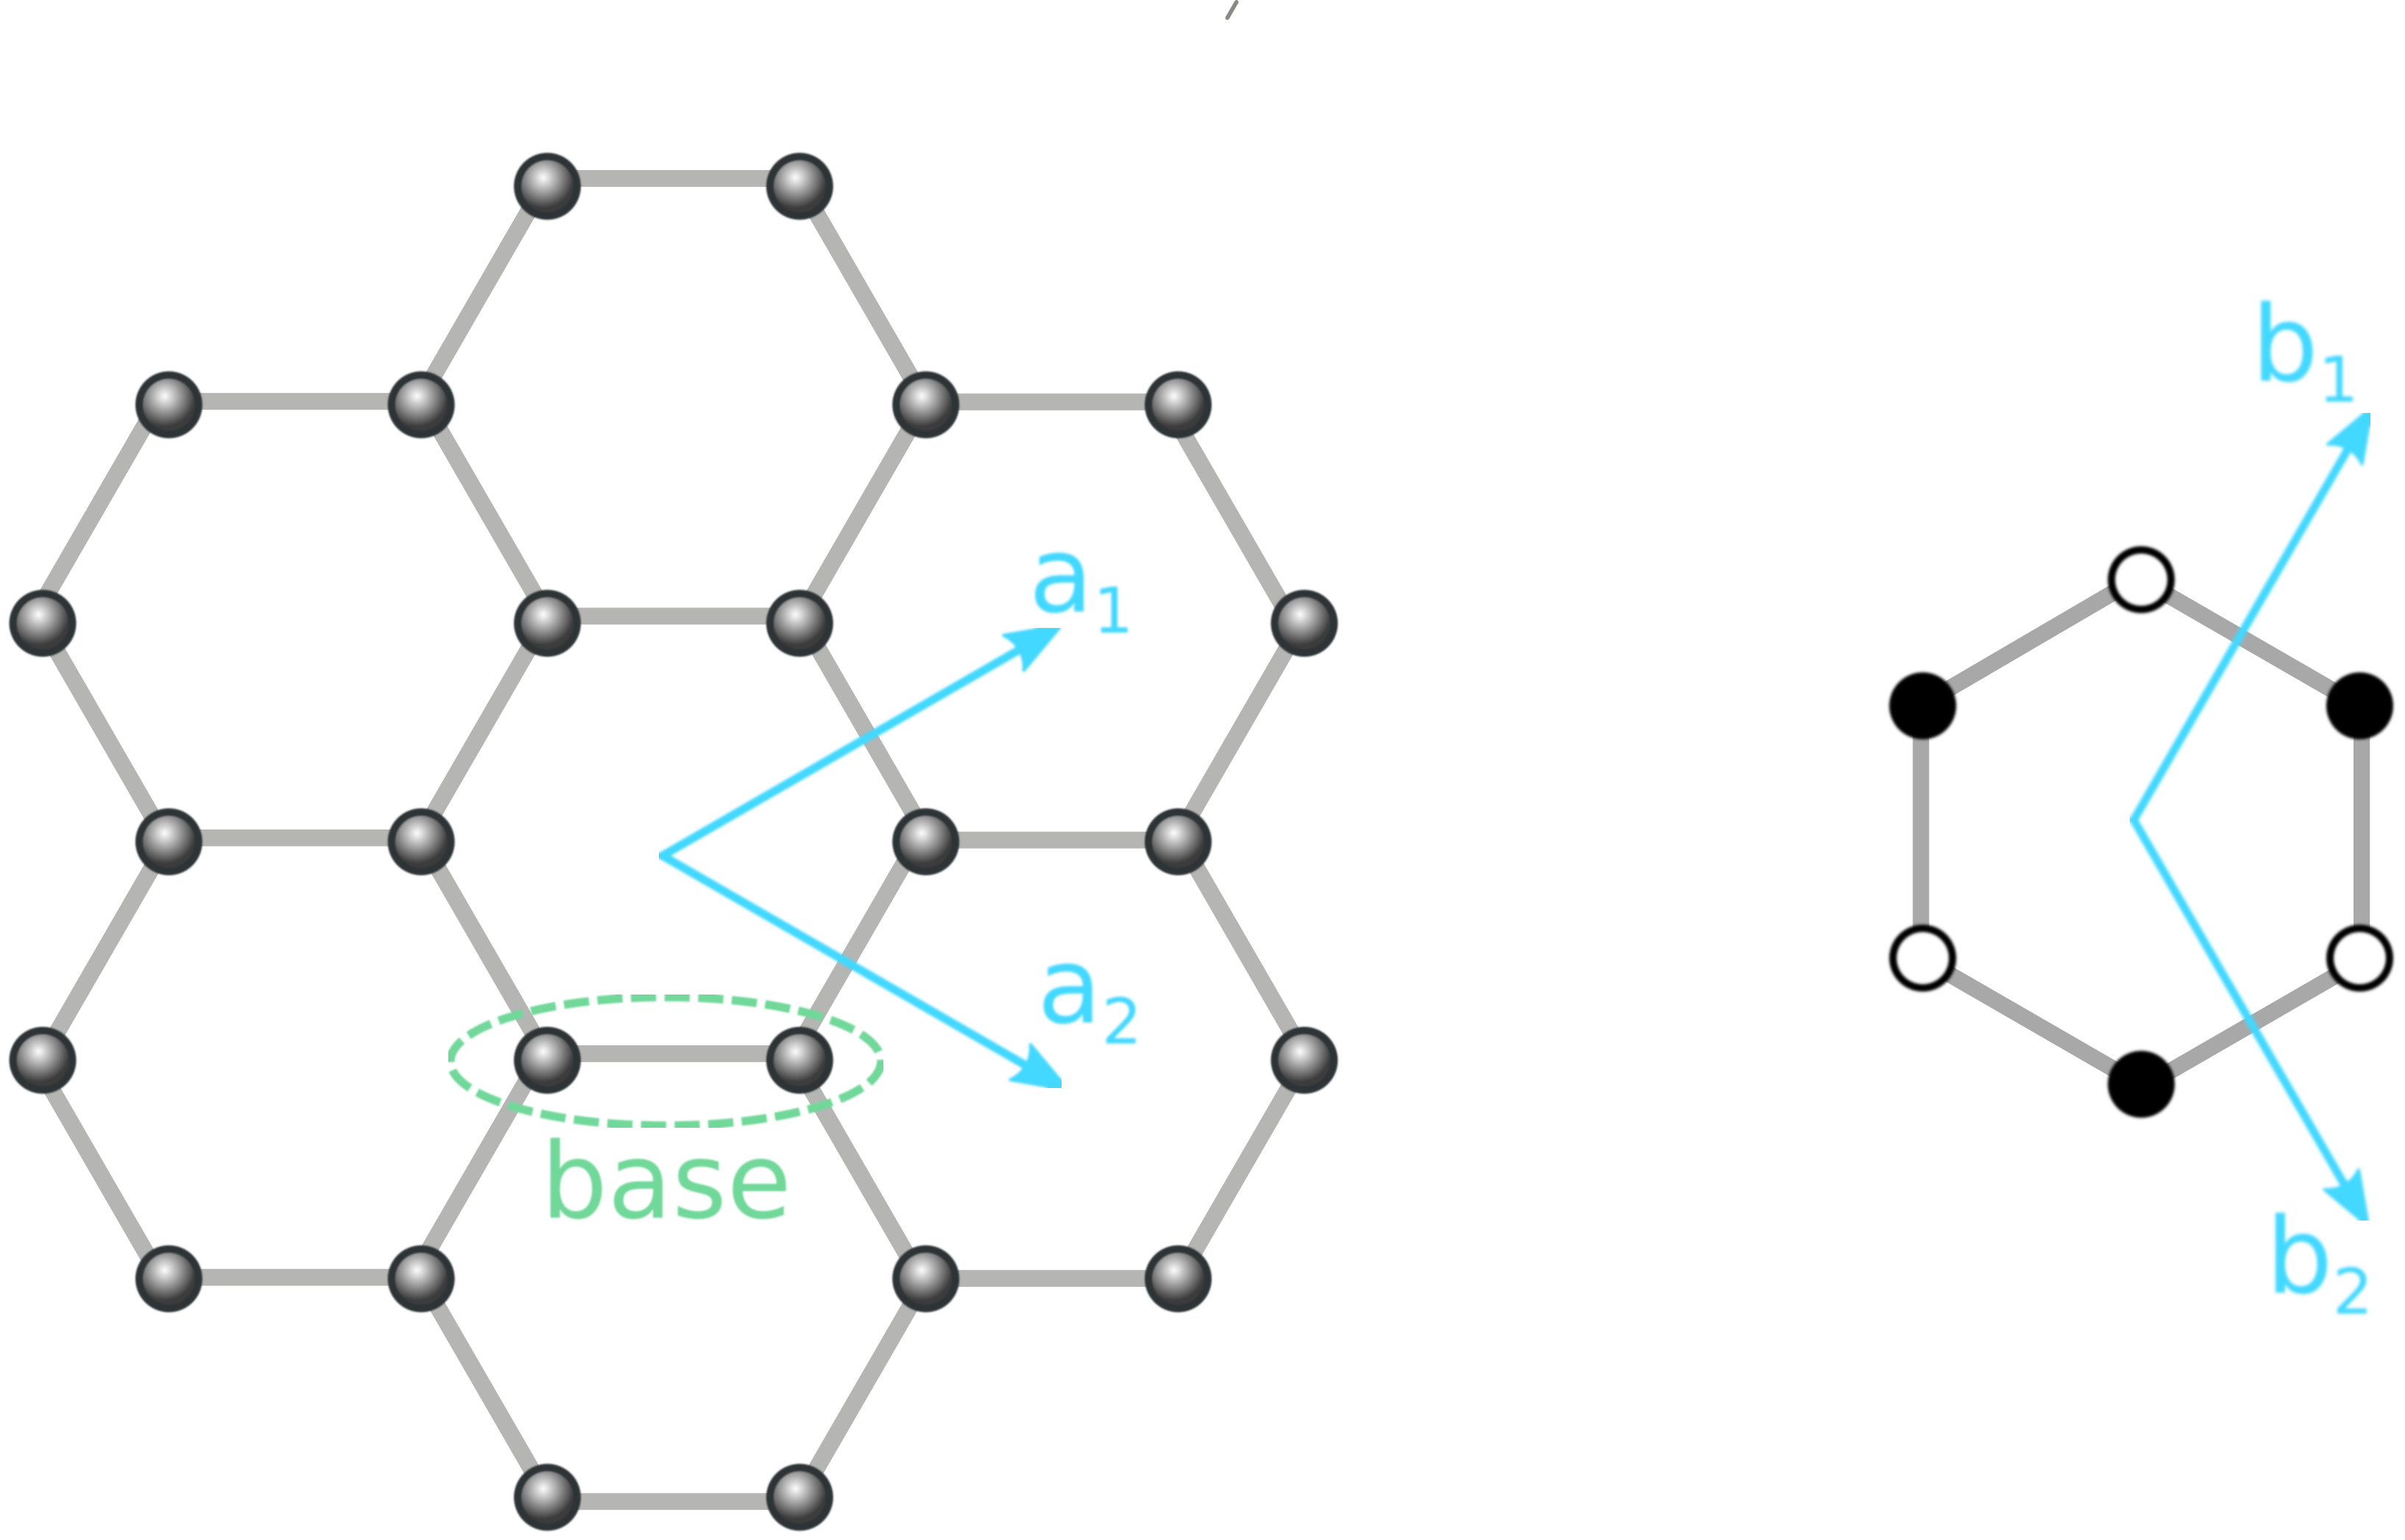
\includegraphics[width=0.75\textwidth]{graphene_lattice.png}
		}
	\caption{Izquierda: Red de grafeno en espacio real. Derecha: Red en espacio recíproco.}
	\label{fig_graphene_lattice}
\end{figure}
El grafeno presenta propiedades extraordinarias, como ha sido demostrado en numerosos experimentos: movilidad electrónica de 200.000 $\mathrm{cm^2 V^{-1} s^{-1} }$ \citep{Bolotin2008}, tensión de ruptura de 130 GPa, y módulo de Young de 1.0 TPa \citep{Lee2008}, conductividad térmica entre 600 a 5000 $\mathrm{W\, mK^{-1}}$ \citep{Balandin2011}, opacidad de 2,3\% y reflectacia menor al 0,1\% \citep{Nair2008}, impermeable totalmente a gases estándar \citep{Bunch2007}, resistir densidades de corriente muy grandes de hasta $\mathrm{10^8 A\, cm^{-2}}$ sin sufrir daños  \citep{Moser2007}, y puede ser funcionalizado fácilmente \citep{Loh2010}. Tiene un área superficial específica calculada de 2630 $\mathrm{m^2 g^{-1}}$ \citep{Peigney2001}. Es importante notar que estos resultados se han obtenido en muestras muy puras de grafeno exfoliado mecánicamente \citep{Novoselov2004} y están lejos de ser replicables a gran escala, se hace necesario encontrar métodos de síntesis que entreguen material de buena calidad (que sus propiedades se acerquen a las citadas anteriormente), y sean escalables a niveles industriales \citep{Novoselov2012}.

\section{Óxido reducido de grafeno (rGO)}
%TODO graphene oxide properties
Una de las formas de obtener grandes cantidades de grafeno es mediante la llamada ruta del "óxido de grafeno". El óxido de grafeno es grafeno decorado densamente por grupos epóxi, hidroxilo, y carboxilo \citep{Dreyer2010}. Los grupos ricos en oxígeno presentes en la red del grafeno se presentan como defectos en éste, cambiando sus propiedades drásticamente.
El óxido de grafeno es sintetizado a partir de grafito natural, exponiéndolo a agentes oxidantes fuertes, esto introduce grupos funcionales ricos en oxígeno en los espacios entre los planos de grafeno del grafito, aumentado la distancia interplanar, y disminuyendo la fuerza entre láminas. Esto facilita la separación de las láminas de grafeno (ahora óxido de grafeno). La mayoría de los métodos de síntesis del óxido de grafeno están basados en alguno de estos tres métodos: método de Brodie \citep{Brodie1859}, método de Staudenmaier \citep{Staudenmaier1898}, o método de Hummers \citep{Hummers1958}.

\begin{figure}
	\centering
	\fbox{
		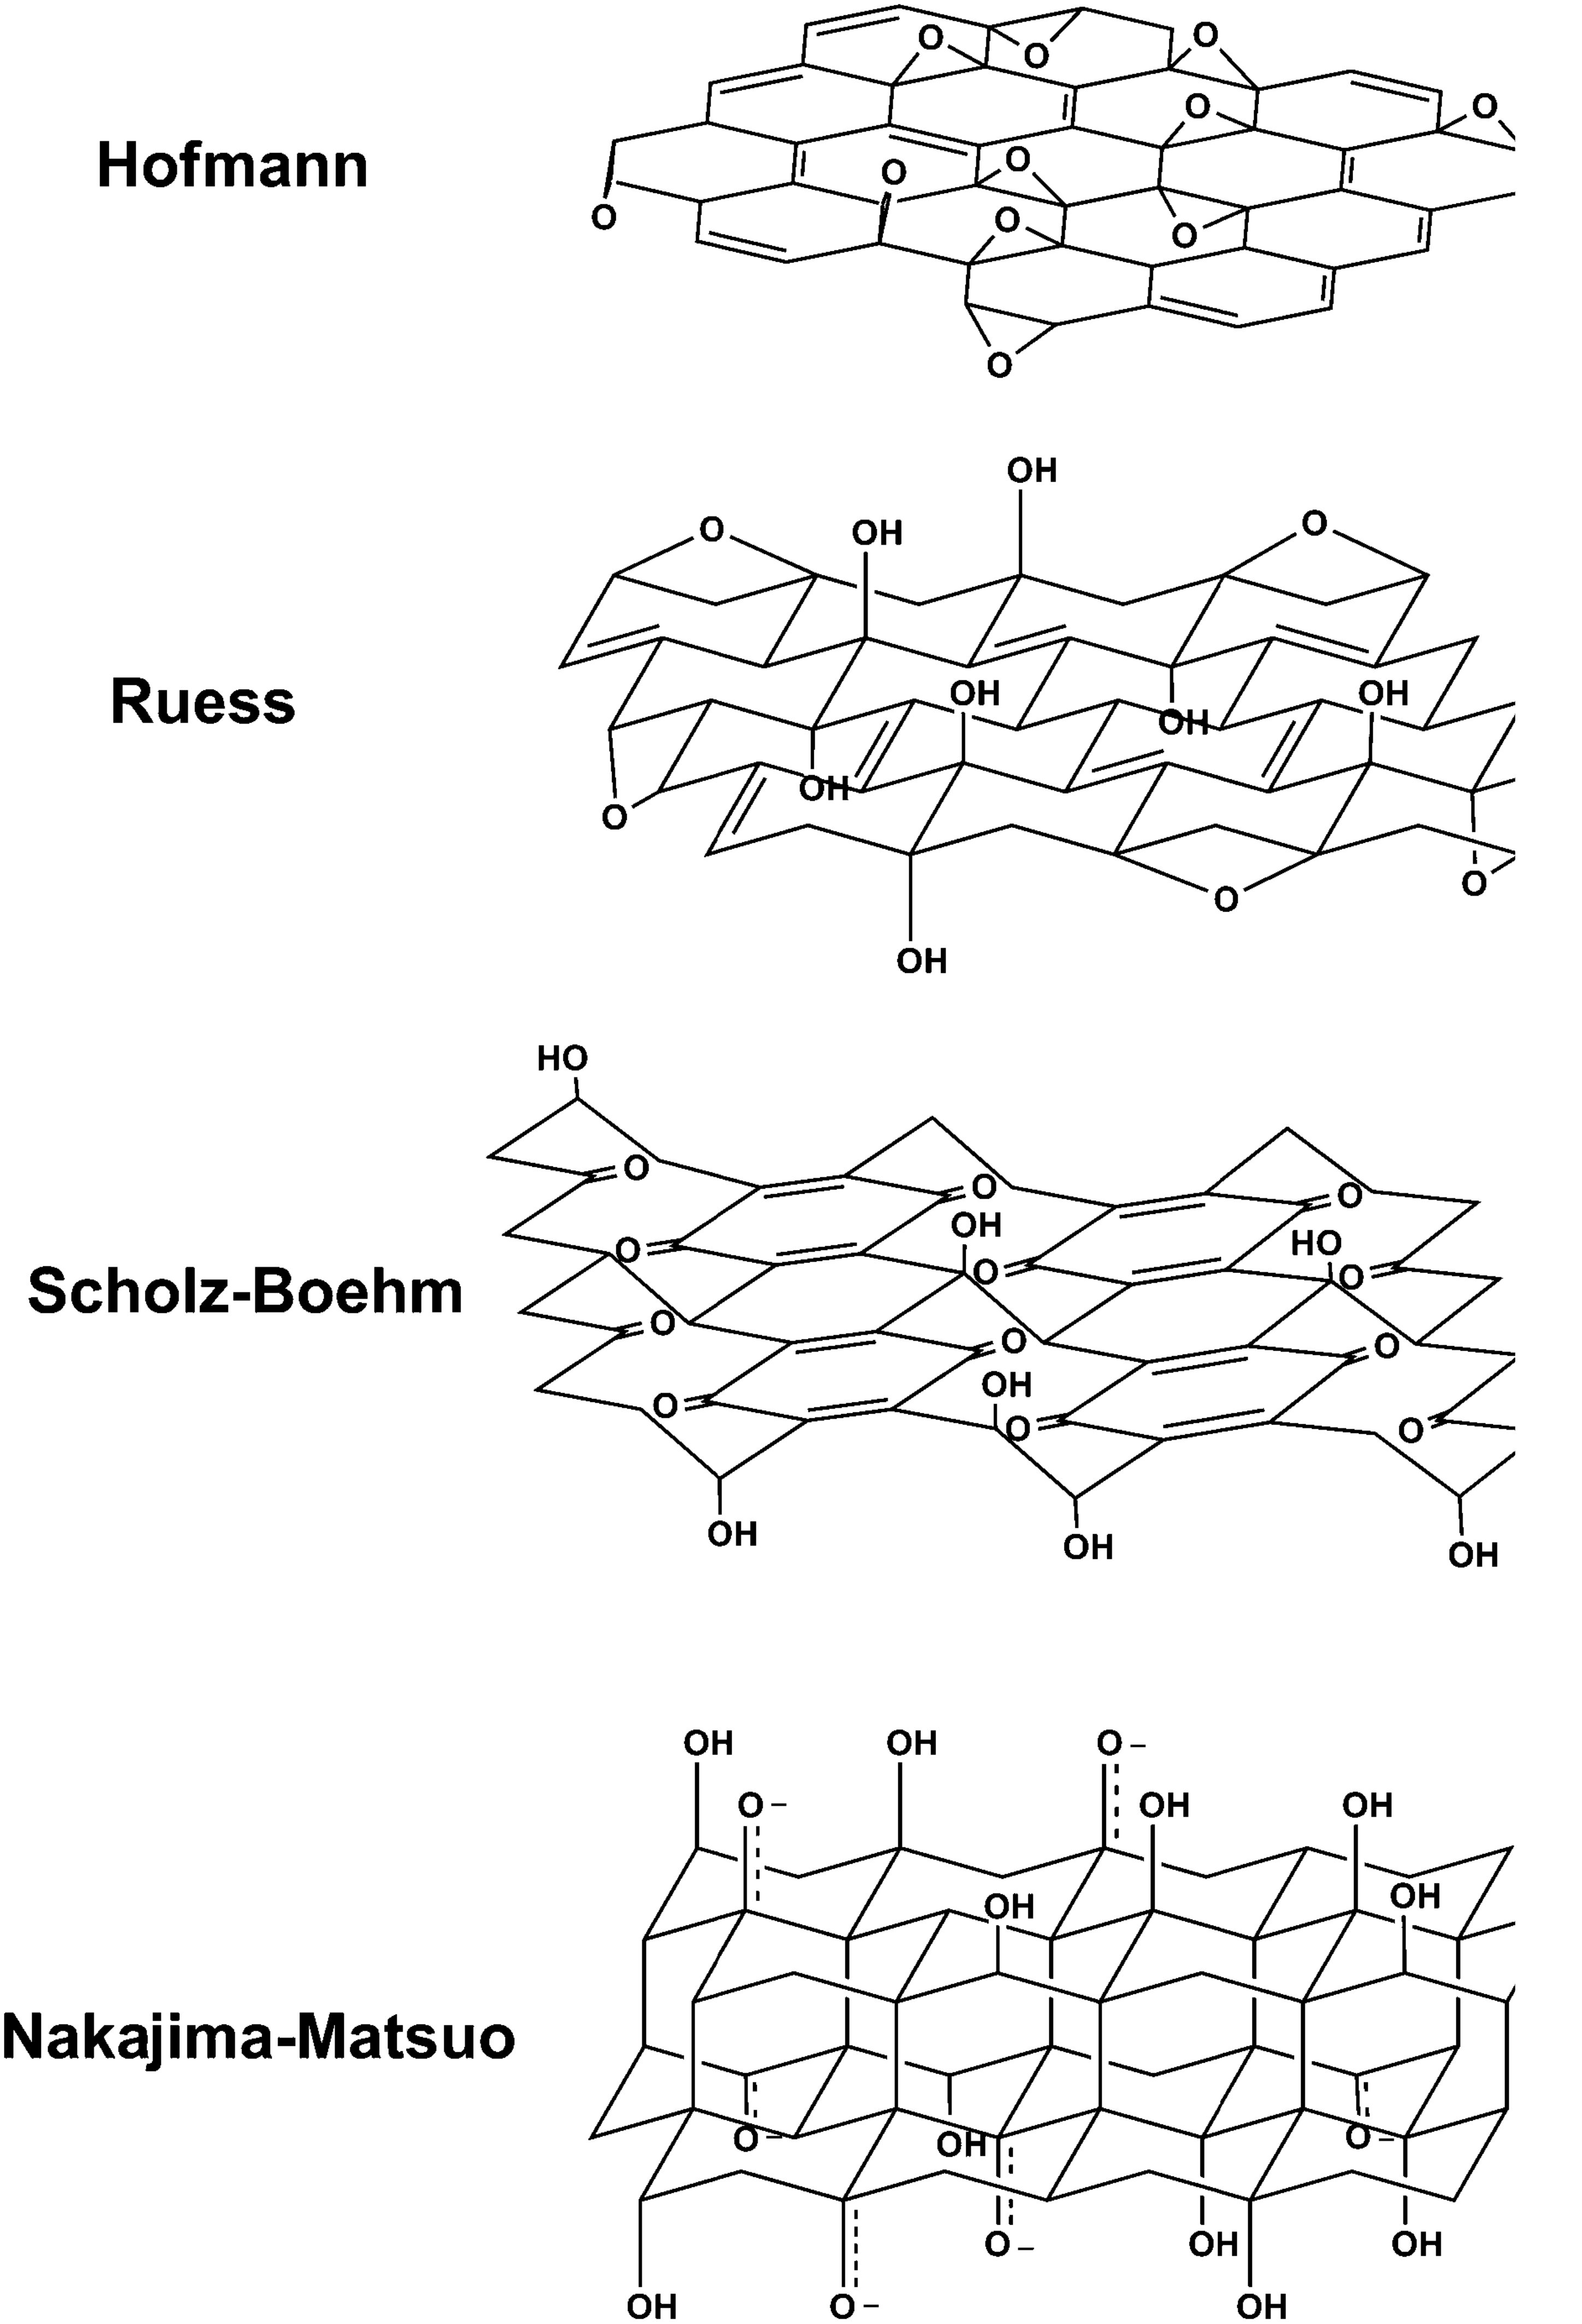
\includegraphics[width=0.5\textwidth]{GO_structure.png}
	}
	\caption{Estructuras propuestas para el óxido de grafeno \citep{Dreyer2010}.}
	\label{fig:GO_structure}
\end{figure}


\section{Síntesis de rGO}
Los grupos funcionales presentes en el óxido de grafeno pueden ser removidos para volver a la estructura del grafeno como tal. Existen muchas formas de reducir el óxido de grafeno, por medios químicos, térmicos, o electroquímicos. En los métodos de reducción química, el óxido de grafeno es expuestos a diferentes agentes reductores, cuyo mecanismo de reducción es sabido, se prueba esperando el efecto deseado \citep{Chua2015}. Por otro lado, la reducción térmica contempla la exposición del óxido de grafeno a altas temperaturas en un horno convencional, reducción por microondas en un horno microondas comercial \citep{Zhu2010a}, reducción por láser \citep{El-Kady2013}, plasma \citep{Lee2012}, o luz solar concentrada \citep{Mohandoss2017}. La reducción electroquímica se realiza en presencia de un solvente, el óxido de grafeno puede estar disperso en el solvente \citep{Liu2011}, depositado en un electrodo \citep{Harima2011, Toh2014}, o bien actuar como electrodo por sí mismo \citep{Feng2016}. Una gran ventaja de los métodos electroquímicos es la facilidad de realizar electrodeposición del rGO en otro electrodo y la combinación con otros nanomateriales, por ejemplo, en una síntesis \emph{in-situ} \citep{Liu2011, Xie2014}.

\section{Aplicaciones}
El óxido reducido de grafeno encuentra su lugar en aplicaciones que requieran gran cantidad de material, en donde los métodos para obtener grafeno de alta calidad simplemente no dan abasto para

%ENERGY APPLICATIONS

%BIOMEDICAL APPLICATIONS

%SENSING APPLICATIONS


\chapter{Supercondensadores}
	%\chapter{Supercondensadores}
\noindent
\rule{\linewidth}{1 pt}
\begin{flushright}
	\begin{quotation}
		\small{
			\textit{``The force is strong with this one.''}}
	\end{quotation}
	\bf{Darth Vader}
\end{flushright}
\noindent
\rule{\linewidth}{1 pt}\\
\vfill

%ENERGY STORAGE
El almacenar energía eléctrica es uno de los mayores problemas a la hora de diseñar sistemas electrónicos tanto móviles como estacionarios, los requerimientos varían de acuerdo a las necesidades de cada uno, en general es un \textit{trade-off} entre densidad de energía (cuánta energía se puede almacenar) y densidad de potencia (que tan rápido puede ser entregada la energía almacenada). Las celdas de combustible (\textit{Fuel Cells}), entregan la mayor densidad de energía, pero son complicadas, mientras que las baterías poseen mayor densidad de potencia, pierden capacidad con los ciclos de carga y descarga. Los supercondensadores van un paso más allá, aumentado la densidad de potencia y aportando mayor vida útil, entregando una nueva posibilidad a la hora de diseñar sistemas eléctricos, ya como fuente de energía por sí mismo, o en sistemas híbridos combinados con otras tecnologías\cite{Thounthong2009}.
\section{El condensador ideal\index{condensador ideal}}
Generalmente un condensador se modela como un par de placas paralelas separadas por un dieléctrico, es definido por su capacitancia, la que refleja la capacidad de almacenar energía. Del modelo de placas paralelas se desprende la definición de capacitancia $C$ como la razón entre la magnitud de carga en cada placa $Q$ y el voltaje entre los terminales $V$:

\begin{equation}
	C = \frac{Q}{V}
\end{equation}

Para fines prácticos, el condensador ideal como componente electrónico es modelado por la ecuación que relaciona la corriente con el voltaje, considerando que $i = dq/dt$:

\begin{equation}
	i(t) = C \frac{dv(t)}{dt}
\end{equation}

Para corrientes constantes, el voltaje varía linealmente como en la carga y descarga de la figura \ref{fig:plot:charge-discharge_ideal_cap}.
\begin{figure}[h!]
	\fbox{
		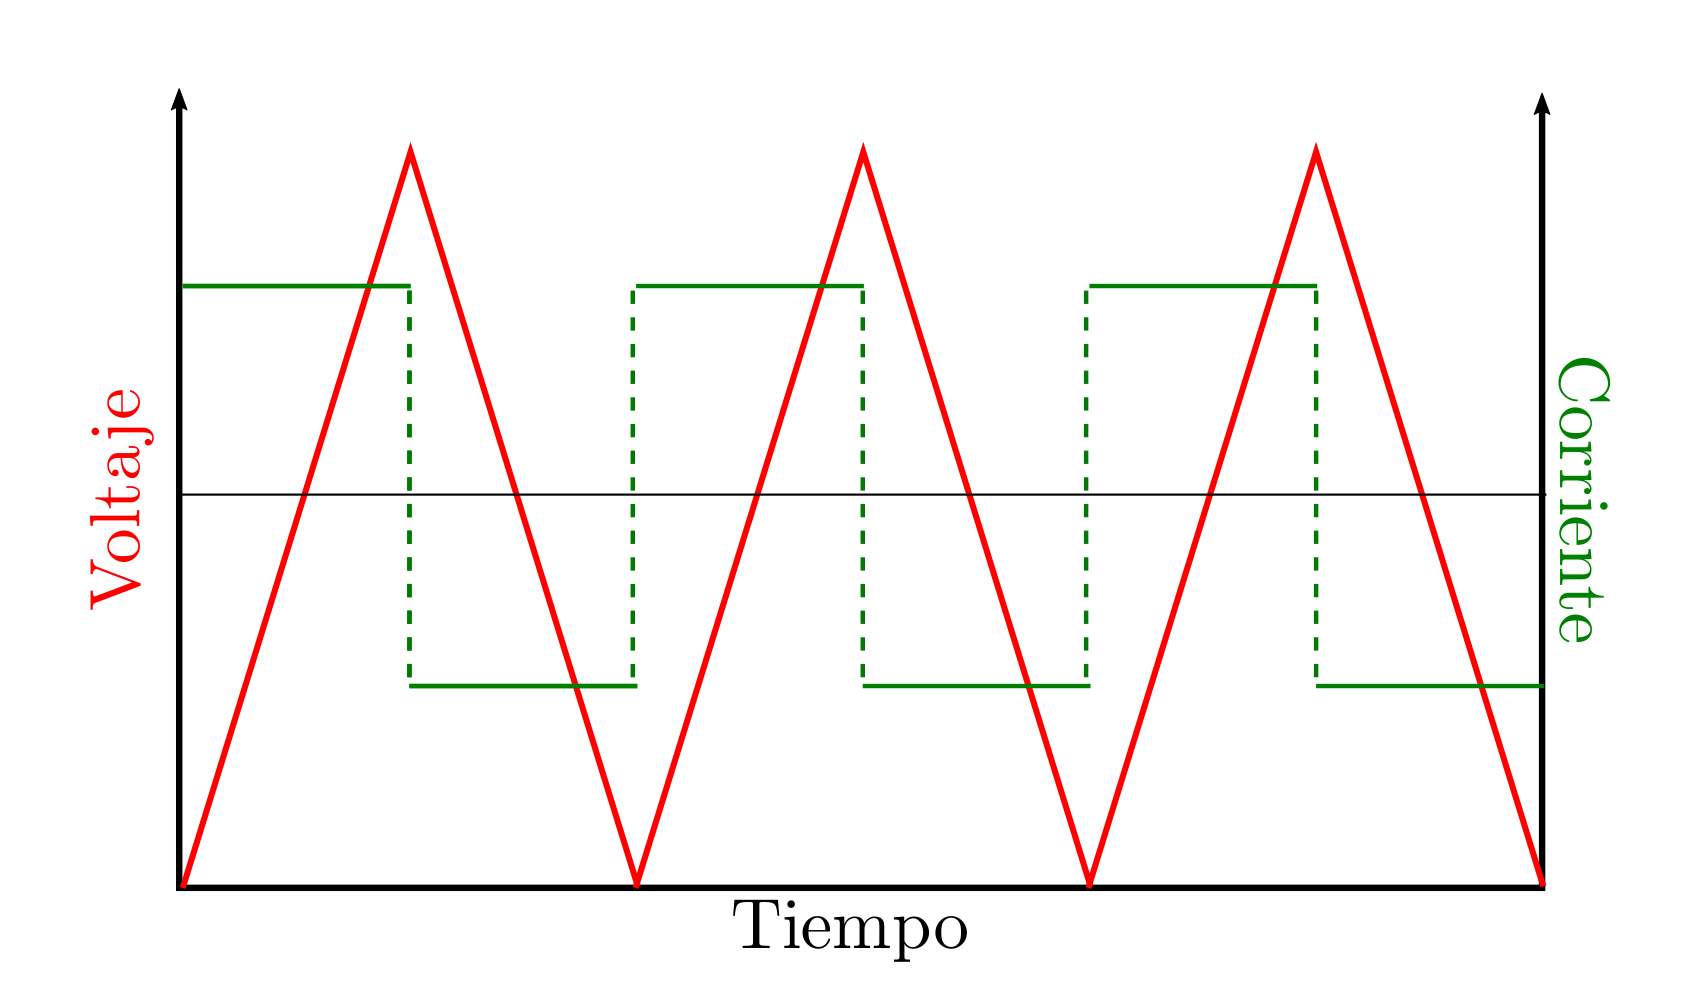
\includegraphics[width=\textwidth]{charge-discharge_ideal_cap.png}
		}
	\caption{Carga y descarga de un condensador ideal a corriente constante.}
	\label{fig:plot:charge-discharge_ideal_cap}
\end{figure}

\section{El condensador real\index{condensador real}}
Un condensador ideal almacenaría energía al cargase y la entregaría al descargarse sin ninguna disipación, es decir, su eficiencia sería del 100\%, podría soportar cualquier voltaje aplicado o cargarse y descargarse por una corriente cuan grande se desee.  En realidad, los condensadores sí disipan energía, poseen voltajes de operación y corrientes máximas de carga y descarga. Todo esto depende de la naturaleza de su construcción y por su puesto, del propósito que fue diseñado.

\subsection{Breakdown voltage}
Los condensadores convencionales construidos con materiales dieléctricos están sujetos a un voltaje máximo de operación determinado por la tensión de ruptura (\textit{Breakdown voltage})\index{tensión de ruptura, \textit{breakdown voltage}}, voltaje al cual se pierden las propiedades dieléctricas del material ocasionando cortocircuito al interior del dispositivo, determinado por la fuerza dieléctrica del material y el espesor de este. En los condensadores electrolíticos la tensión de ruptura es determinada por otros mecanismos\cite{Yahalom1971}. En lo que respecta a los supercondensadores, el voltaje máximo de carga depende fundamentalmente de electrolíto usado, principalmente por las reacciones que ocurren a ciertos potenciales, este tema será abordado con más detalle en la sección correspondiente.

\subsection{Circuito equivalente}
El comportamiento de los condensadores reales son modeladas por un circuito equivalente, donde se introducen componentes que representan las imperfecciones del funcionamiento del condensador real.\\

\subsection{Resistencia en serie equivalente (ESR)}
Las imperfecciones en la construcción de los electrodos, y la naturaleza de los materiales utilizados (e.g. resistencia no cero), disipan energía durante la carga y descarga como si se tratase de una resistencia en serie al condensador, esto se ve reflejado como una caída de voltaje en los terminales del dispositivo (figura \ref{fig:plot:charge-discharge_esr}), y disminuye la eficiencia de éste.

\begin{figure}[h!]
	\fbox{
		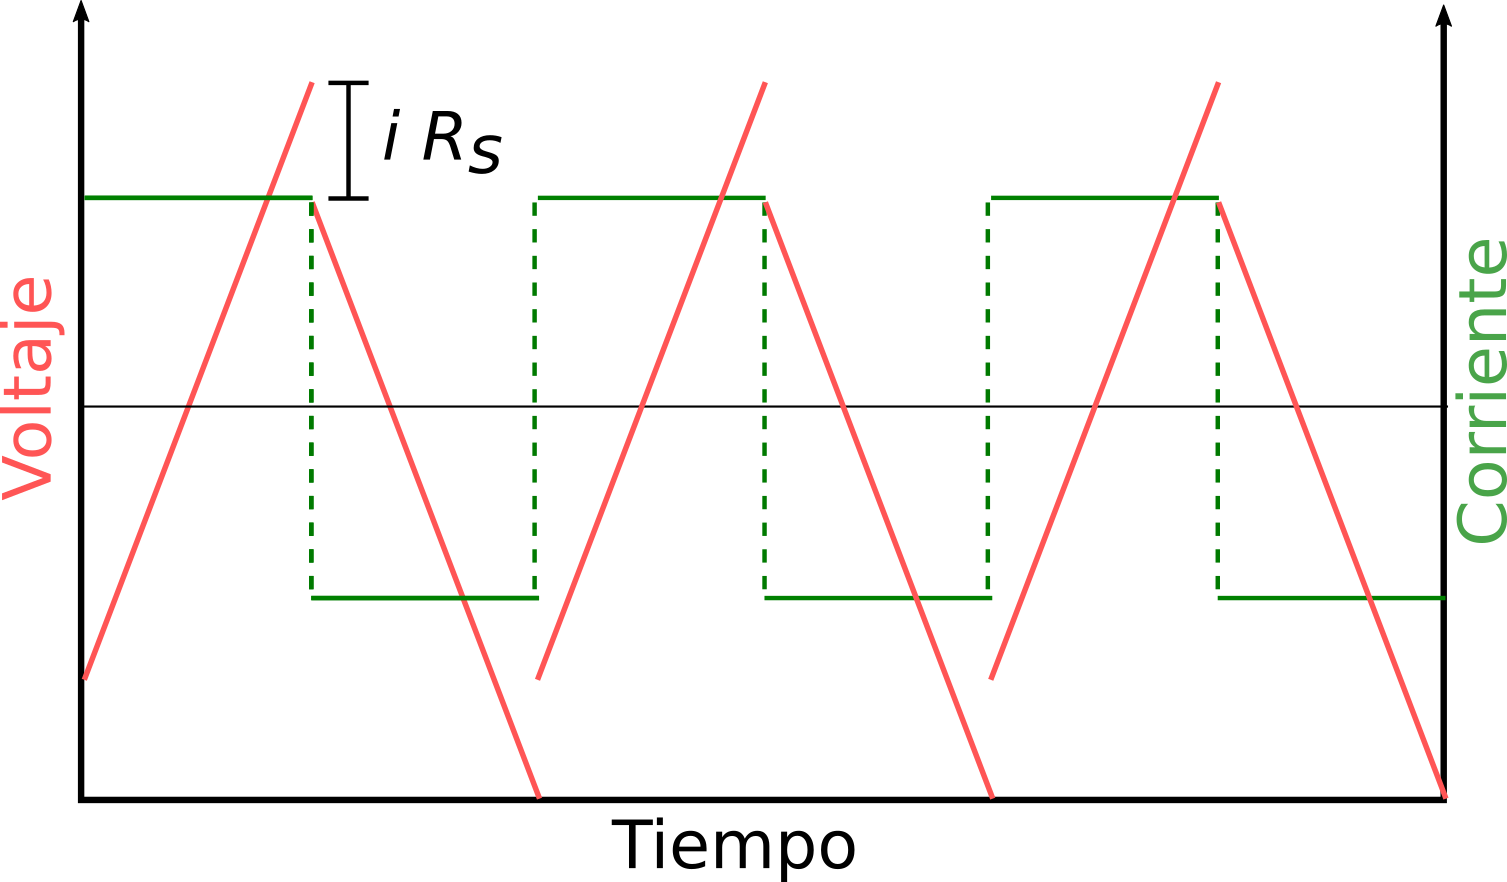
\includegraphics[width=\textwidth]{charge-discharge_esr.png}
	}
	\caption{Carga y descarga de un condensador evidenciando el efecto de una ESR.}
	\label{fig:plot:charge-discharge_esr}
\end{figure}

\subsection{Corriente de fuga (\emph{leakage current})}
Entre los electrodos del condensador fluye una corriente no deseada cuando existe una diferencia de potencial entre los electrodos, esta corriente 

\section{¿Qué hace a un supercondensador?}

\subsection{Doble capa electrostática de Helmholtz}

\subsection{Pseudocapacitancia}
\chapter{Síntesis de óxido de grafeno}
%Chapter{Sintesis de óxido de grafeno}
El método de síntesis utilizado está basado en el propuesto por Hummers para la síntesis de óxido de grafito \citep{Hummers1958}, y es descrito por Abdolhosseinzadeh \citep{Abdolhosseinzadeh2015}, la principal diferencia con el procedimiento original de Hummers, es la introducción de etapas de sonicación para asistir en la exfoliación del óxido de grafito.

\section{Procedimiento experimental}
En una síntesis normal 1 g de grafito en polvo (Sigma-Aldrich $>$99\%) o en hojuelas (Superior Graphite $>$80\%), tal como viene envasado, se añaden a 50 ml de ácido sulfúrico (\ce{H_2SO_4}, Baker 97.8\%) en un vaso precipitado de 250 ml previamente puesto en un baño de hielo sobre un agitador magnético, la mezcla se deja agitar por 5 minutos. Una vez el grafito se ha dispersado en el ácido sulfúrico se agregan 3 g de permanganato de potasio (\ce{KMnO_4}, Chemix 99.44\%), lentamente, manteniendo la temperatura de la mezcla bajo los 10 C y así evitar la explosión del permanganato. Luego de 15 minutos de agitación, se quita del baño de hielo y se agita 25 minutos más a temperatura ambiente, seguido de 5 minutos en un baño ultrasónico (99\% de potencia, SB-3200DTD Ultrasonic Cleaner), este proceso de agitación-sonicación es repetido 12 veces, tomando un total de 6 horas en completarse. Una vez completado este proceso, se agregan 200 ml de agua destilada rápidamente, esto produce una reacción exotérmica con evolución de gases, la solución se vuelve marrón, color característico del óxido de grafeno. En general, la solución se divide en dos partes iguales, y se vuelven a sonicar por dos horas más, una de las partes es reducida posteriormente, mientras que la otra se trata con agua oxigenada (\ce{H_{2}O_2}) tal como lo menciona Hummers en su escrito original, para reducir el permanganato y dióxido de manganato restante en la solución \citep{Hummers1958}, 20 ml de \ce{H_2O_2} al 30\% se añaden lentamente mientras se continúa la  agitación, la solución se vuelve de color amarillo brillante al agregar el peróxido de hidrógeno y libera gases. Cuando la evolución de gases cesa, se remueve del agitador magnético y se deja a temperatura ambiente, transcurrido un día de reposo, el material precipita al fondo del vaso, y se procede a remover el resto de la solución acuosa que contiene restos de la reacción para luego rellenar el vaso con agua destilada, este proceso de lavado es realizado al menos cuatro veces y por último se remueve la mayor cantidad de agua, para dejarlo secar a temperatura ambiente.

\section{Resultados}
Del proceso de síntesis anterior se obtienen dos resultados, el óxido de grafeno lavado con peróxido de hidrógeno y lavado, y otro sin lavar que es utilizado para su posterior reducción.

El óxido de grafeno lavado con \ce{H_{2}O_2} es de color marrón claro y una vez seco se oscurece con el pasar de los días.

\begin{figure}
	\centering
	\fbox{
		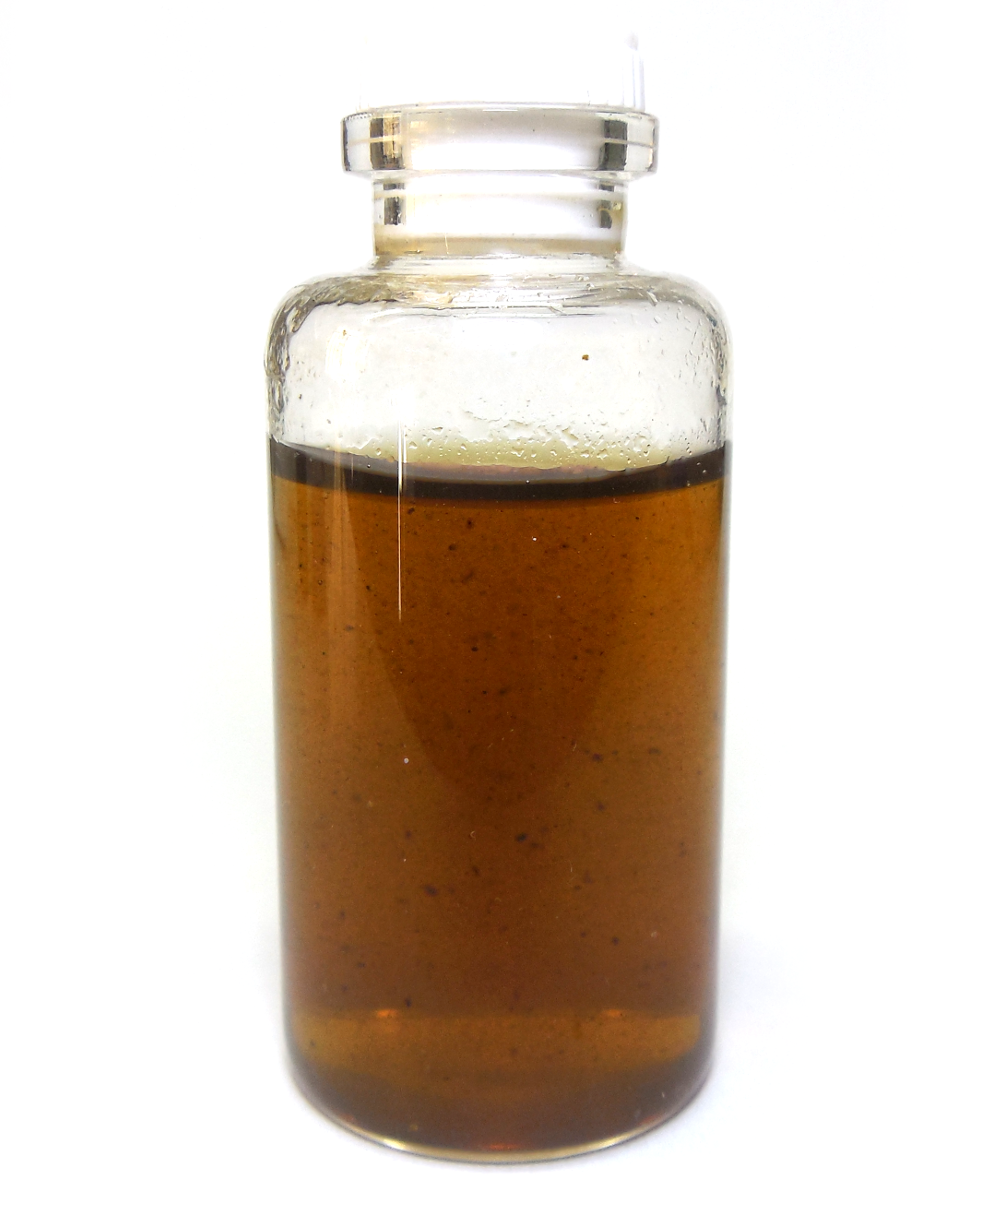
\includegraphics[width=0.5\textwidth]{GO_pic.png}
	}
	\caption{GO}
	\label{fig:GO}
\end{figure}

El óxido de grafeno es caracterizado por espectroscopía de rayos x (XRD), UV-Vis, y microscopia SEM.

\begin{figure}
	\centering
	\fbox{
		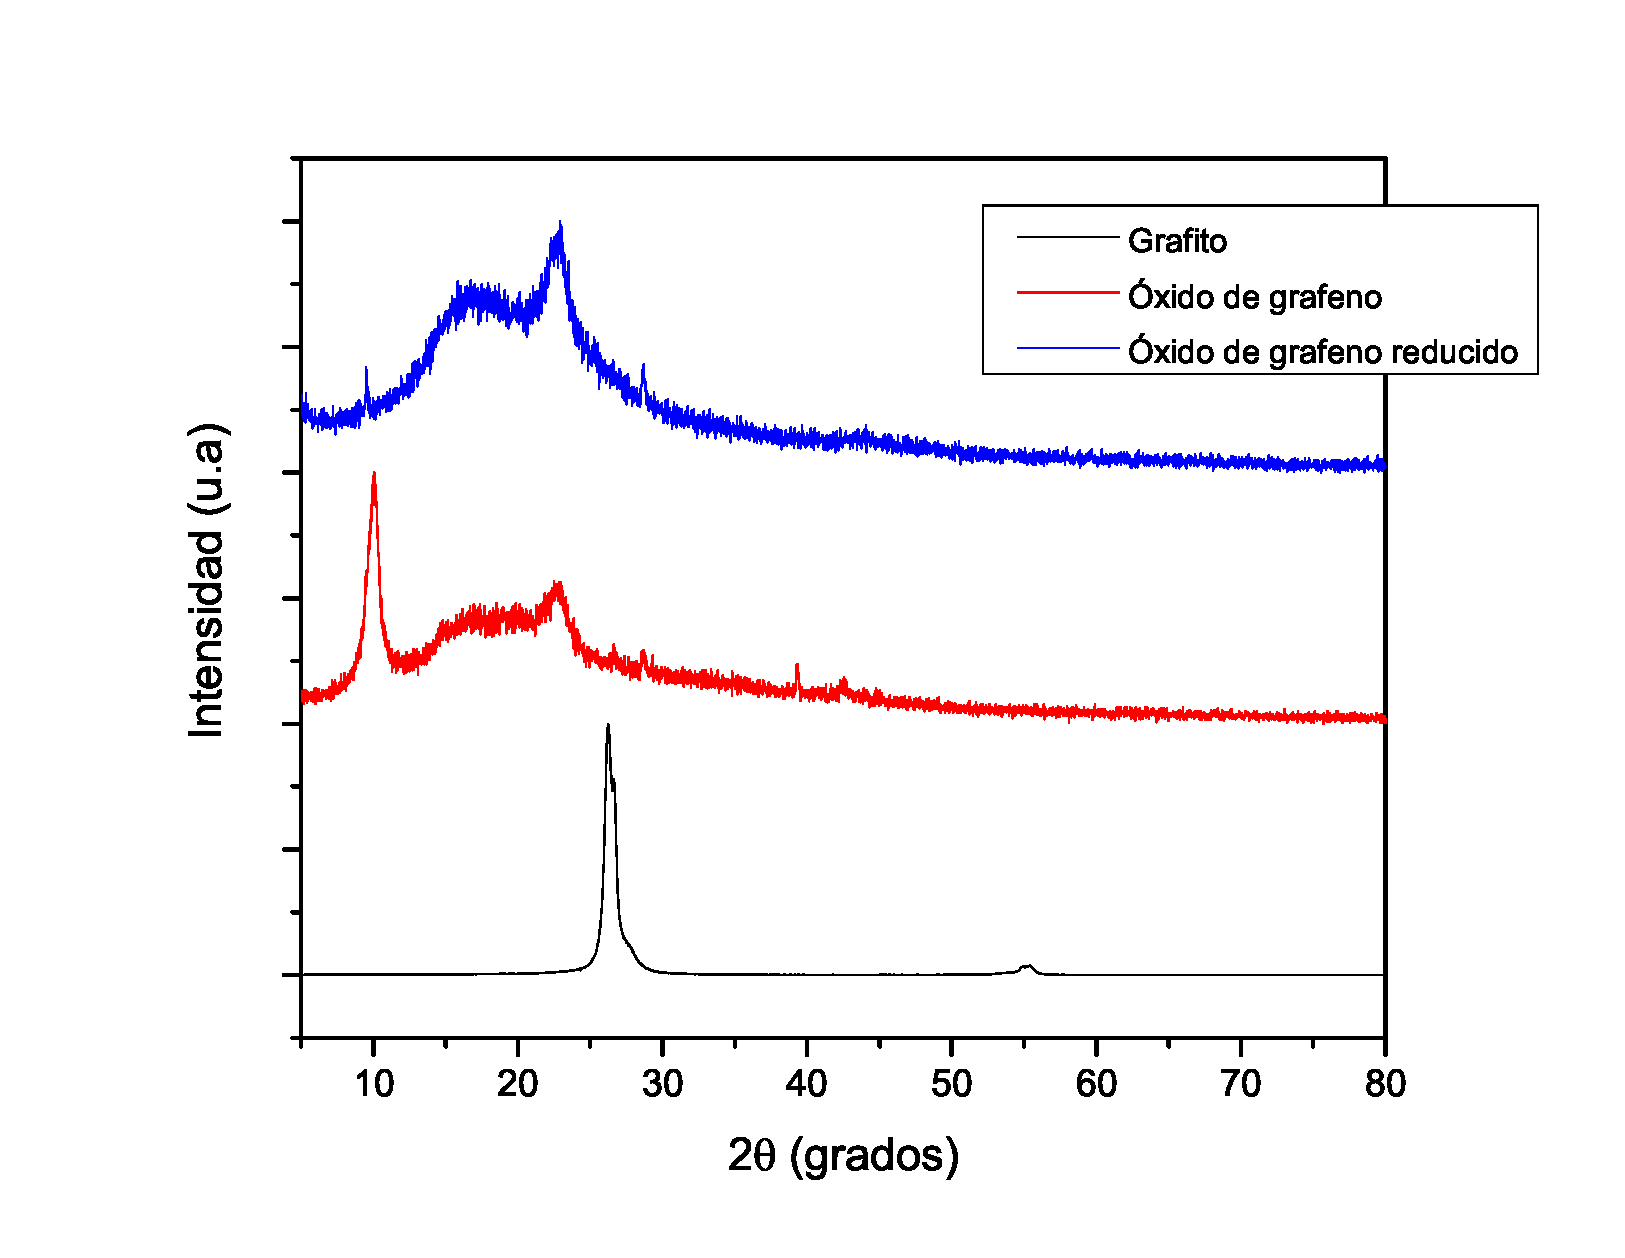
\includegraphics[width=1\textwidth]{../Data/Resumen.eps}
	}
	\caption{Espectro óxido de grafeno.}
	\label{fig:xrd_GO}
\end{figure}
\chapter{Reducción del óxido de grafeno}

\section{Materiales}
Como precursor se usa el óxido de grafeno sintetizado con anterioridad mediante el método de Hummers
\section{Procedimiento}

\section{Resultados}
\chapter{Construcción de supercondensadores}
%\chapter{Construcción de supercondensadores}
Un supercondensador es construido haciendo el sándwich electrodo-separador-electrodo, más la adición de un electrolito. Este último, es una solución acuosa de hidróxido de potasio (\ce{KOH}), a una concentración 6M; esta es utilizada ampliamente en este tipo de estudios \citep{Frackowiak2001}.  El material que servirá de electrodo debe estar depositado en un colector de corriente, o bien ser una lámina libre. Por otro lado, el separador es una membrana permeable al electrolito, el cual puede ser una membrana microporosa o papel filtro de celulosa. Este último es el empleado en esta tesis.

La primera aproximación a la construcción del supercondensador se explica en la secuencia de la figura \ref{fig:SC_process}. Primero se adhiere el colector de corriente metálico a un sustrato de vidrio. Segundo, se delimita el área a depositar mediante una cinta adhesiva. Tercero se deposita mediante goteo la dispersión de óxido de grafeno reducido en el colector de corriente. Cuarto, se evapora el líquido dispersante. Quinto, se añaden gotas de electrolito al separador de celulosa. Sexto, se cierra el sistema con un segundo electrodo.

\begin{figure}[h!]
	\centering
	\fbox{
		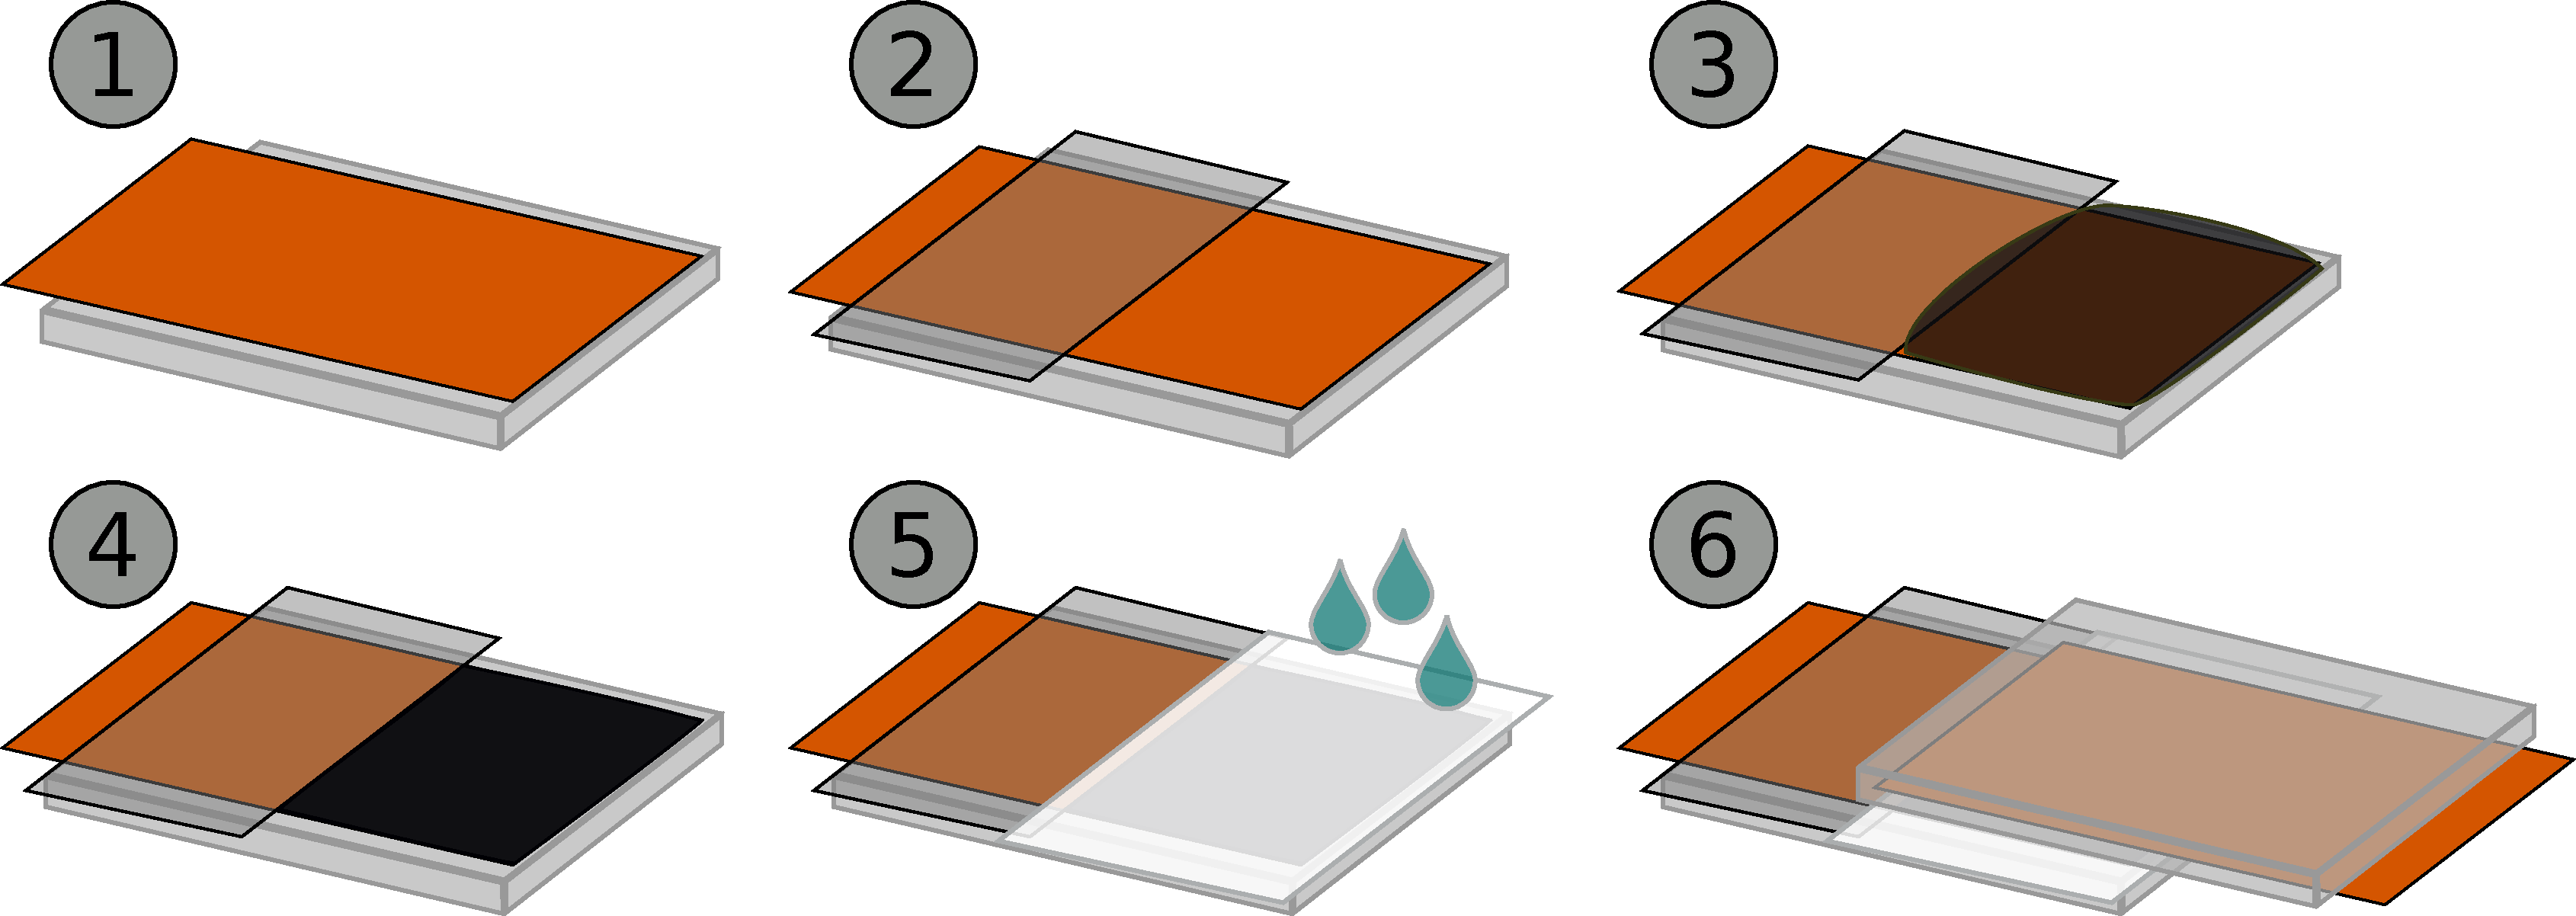
\includegraphics[width = 0.9\textwidth]{SC_process.pdf}
		}
	\caption[Principio de contrucción de un supercondensador]{Secuencia para la construcción de un supercondensador básico.}
	\label{fig:SC_process}
\end{figure}

\section{Celda de prueba de supercondensador}
La construcción de supercondensadores, como se detalla anteriormente, presenta varios inconvenientes: (1) Los colectores de corriente de aluminio y cobre utilizados, se degradan rápidamente al exponerse al electrolito (KOH), y son propensos a reacciones redox. (2) La deposición de material en los colectores de corriente no es homogénea, generando zonas donde el colector queda expuesto al electrolito. (3) El agua del electrolito se evapora rápidamente, disminuyendo la cantidad de iones en el medio de conducción. (4) El cierre del dispositivo no es estable y no permite su reproducibilidad, y por consiguiente (5) La conexión a los terminales eléctricos no es estable. Por estas razones y conservando los principios básicos de la construcción de supercondensadores, se diseña una celda de pruebas para solucionar estos problemas.

La celda diseñada y construida (figura \ref{fig:celda_de_pruebas_SC}), consta de dos colectores de corriente de acero inoxidable, entre los que se ubica el supercondensador. Los colectores de corriente tienen juntas tóricas que impiden la fuga del electrolito o la evaporación del agua en él, permitiendo una operación estable en el tiempo. Los colectores de corriente se apoyan en bloques de acero que aseguran la celda con cuatro pernos, permitiendo conectar los terminales del potenciostato a la celda de pruebas.

\begin{figure}[h!]
	\centering
	\fbox{
	\begin{subfigure}[b]{0.5\textwidth}
		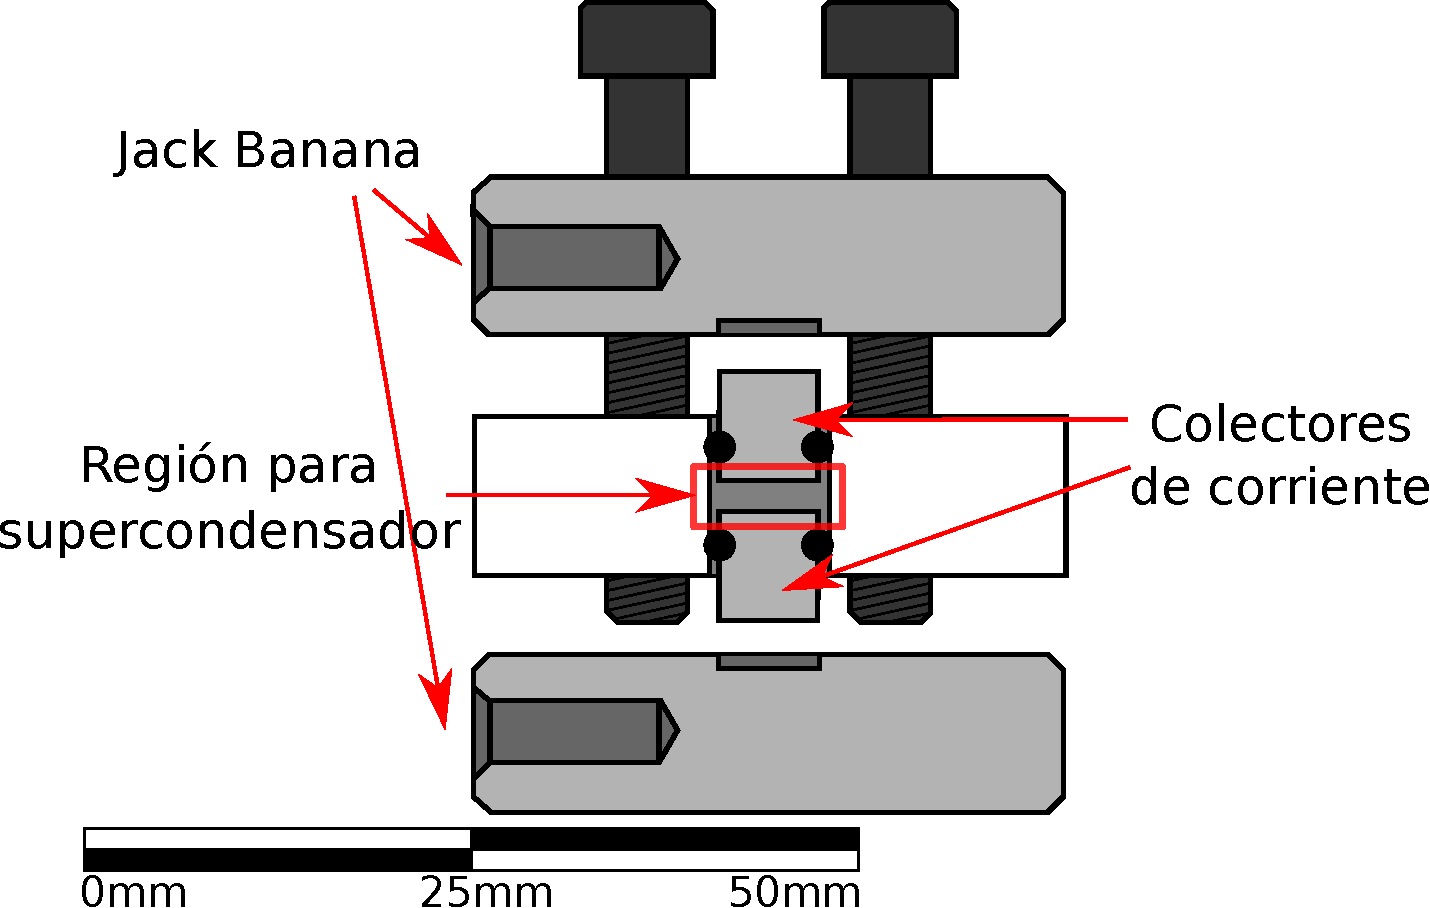
\includegraphics[width=\textwidth]{cell_scheme.pdf}
		\caption{}
		\label{fig:cell_scheme}
	\end{subfigure}\hspace{1cm}
	\begin{subfigure}[b]{0.25\textwidth}
		\includegraphics[width=\textwidth]{cell_image.pdf}
		\caption{}
		\label{fig:cell_image}
	\end{subfigure}
	}
	\caption[Celda de prueba de supercondensador]{\subref{fig:cell_scheme} Vista en corte longitudinal de la celda de pruebas mostrando los componentes más importantes. \subref{fig:cell_image} Fotografía de la celda armada y conectada al potenciostato.}
	\label{fig:celda_de_pruebas_SC}
\end{figure}

\section{Construcción de electrodos}
Se fabrican seis pares de electrodos utilizando el mismo material sintetizado, pero diferentes sustratos y diferentes métodos de deposión. Se utilizan dos tipos de sustratos, el primero es un disco de acero UNS316L de 7 mm de díametro, el segundo es un disco de espuma de níquel también de 7 mm de diámetro, que tiene mayor área superficial (EQ-bcnf-16m, MTI Corporation). Para fabricar el primer par de electrodos, el material en forma de polvo es dispersado ultrasonicamente en etilenglicol, que mostró mayor homogeneidad que el agua para la deposición de rGO, y depositado por goteo hasta cubrir completamente el sustrato de acero previamente calentado a 150 \degree C. Un segundo par se fabrica añadiendo polimetilmetacrilato (PMMA), a la solución a depositar. Este se disuelve en acetona a una concentración de 10 mg/ml, solución donde se dispersa el óxido reducido de grafeno por medio de ultrasonido y luego es depositada por goteo en el sustrato de acero a 50 \degree C. De forma análoga, el tercer y cuarto par repiten los procesos anteriores pero cambiando el sustrato de acero por el de níquel. Manteniendo el sustrato de acero, el quinto par consiste en electrodos de papel fabricados mediante filtración por vacío. En este método, se dispersa el rGO en agua, la que se pasa por un filtro de celulosa en un embudo Büchner conectado a un kitasato y una bomba de vacío. El filtro con el material atrapado se deja secar a temperatura ambiente formando una lámina, la que es desprendida con facilidad del filtro y luego recortada al tamaño apropiado para la celda de pruebas (7 mm). El material dispersado en agua también puede ser liofilizado, obteniendo una espuma de rGO que es utilizada como electrodo en la celda.
%TODO balanza
La masa del material depositado se mide en una balanza analítica (Radwag Modelo AS 220/C2, resolución 0,1 mg), conociendo previamente la masa de los sustratos y teniendo la precaución que el solvente se haya evaporado totalmente. Para los discos de papel de rGO, se masan 20 de ellos y se calcula la masa promedio de cada uno. En el caso del material liofilizado, se masa directamente la cantidad a utilizar en la celda de pruebas. En la tabla \ref{tab:electrodos_construidos} se resumen los electrodos fabricados, detallando la masa de material activo y en la figura \ref{fig:electrodes} se muestran algunos de estos.

\begin{table}[htbp]
	\centering
	\caption{Electrodos fabricados para supercondensadores.}
	\begin{tabular}{ l l l l l c }
		\multirow{2}{*}{Nombre}	&\multirow{2}{*}{Sustrato} & \multirow{2}{*}{Formato}& \multirow{2}{*}{Aglutinante} & \multirow{2}{*}{Masa [mg]}& Caracterización\\
				&			&				&				&				&  electroquímica \\
		\hline
		\mSustratoAcero		&	Acero    &   -           & -      &  -            & Figura \ref{SCGraphs:CV_Steel_Disk_No_Material_1} \\
		\mPolvoAcero			&	Acero    & Polvo         & -      & 0,4 $\pm$ 0,2 & Figura \ref{SCGraphs:CV_CRGO300517_9}             \\
		\mPolvoAceroPMMA	&	Acero    & Polvo         & PMMA   & 2,8 $\pm$ 0,2 & Figura \ref{SCGraphs:CV_CRGO300517_3}             \\
		\mPapelAcero		&	Acero    & Papel         & -      & 0,6 $\pm$ 0,1 & Figura \ref{SCGraphs:CV_CRGO300517_11}            \\
		\mLiofilizadoAcero	&	Acero    & Liofilizado   & -      & 0,6 $\pm$ 0,1 & Figura \ref{SCGraphs:CV_CRGO300517_13}            \\
		\mSustratoNiquel	&	Níquel   &  -            & -      &    -          & Figura \ref{SCGraphs:CV_Nickel_Foam_No_Material_1}\\
		\mPolvoNiquel		&	Níquel   & Polvo         & -      & 0,9 $\pm$ 0,2 & Figura \ref{SCGraphs:CV_CRGO300517_5}             \\
		\mPolvoNiquelPMMA	&	Níquel   & Polvo         & PMMA   & 0,8 $\pm$ 0,2 & Figura \ref{SCGraphs:CV_CRGO300517_7}             \\
	\end{tabular}
	\label{tab:electrodos_construidos}
\end{table}

\newcommand{\electrodesWidth}{0.22\textwidth}
\begin{figure}
	\centering
	\begin{adjustbox}{minipage=\linewidth,frame}
	\centering
		\begin{subfigure}[b]{\electrodesWidth}
			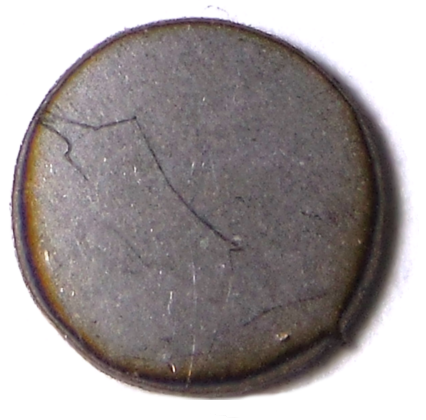
\includegraphics[width=\textwidth]{electrode_steel.png}
			\caption{\mSustratoAcero}
			\label{fig:substrate_steel}
		\end{subfigure}
		\begin{subfigure}[b]{\electrodesWidth}
			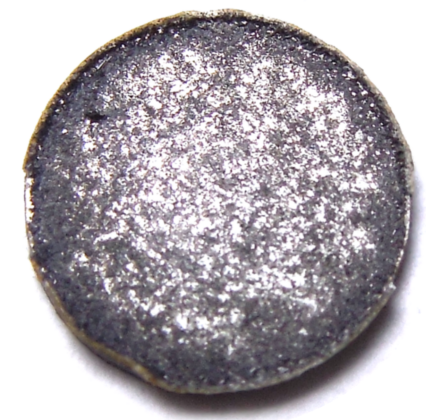
\includegraphics[width=\textwidth]{electrode_polvo_ac.png}
			\caption{\mPolvoAcero}
			\label{fig:electrode_powder_ac}
		\end{subfigure}
		\begin{subfigure}[b]{\electrodesWidth}
			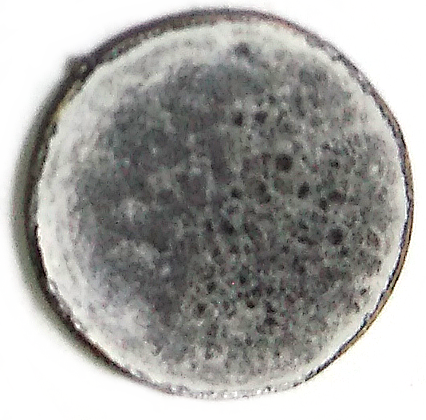
\includegraphics[width=\textwidth]{electrode_polvo_pmma_ac.png}
			\caption{\mPolvoAceroPMMA}
			\label{fig:electrode_powder_pmma_ac}
		\end{subfigure}
		\begin{subfigure}[b]{\electrodesWidth}
			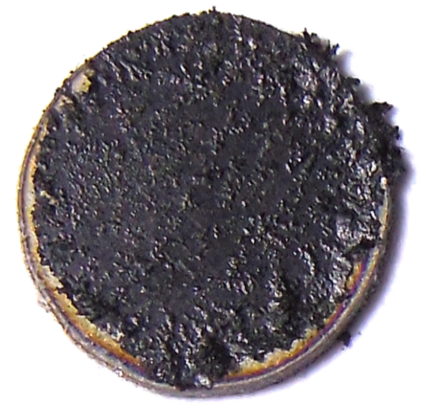
\includegraphics[width=\textwidth]{electrode_paper.png}
			\caption{\mPapelAcero}
			\label{fig:electrode_paper}
		\end{subfigure}\linebreak
		\begin{subfigure}[b]{\electrodesWidth}
			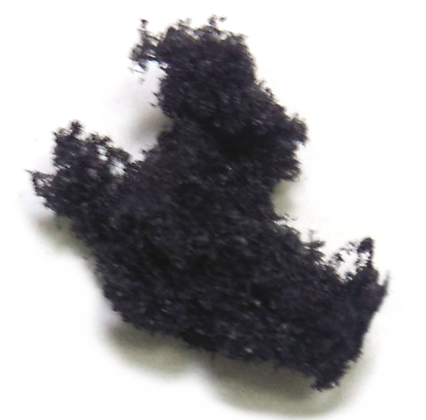
\includegraphics[width=\textwidth]{electrode_lio.png}
			\caption{\mLiofilizadoAcero}
			\label{fig:electrode_lio}
		\end{subfigure}
		\begin{subfigure}[b]{\electrodesWidth}
			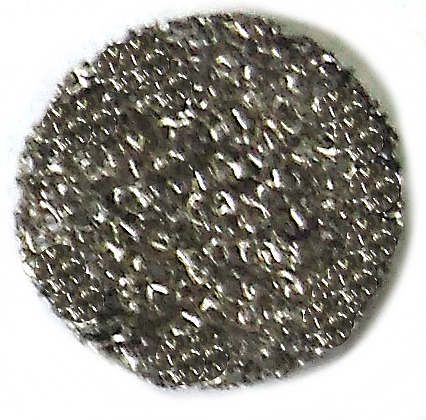
\includegraphics[width=\textwidth]{electrode_ni.png}
			\caption{\mSustratoNiquel}
			\label{fig:substrate_nickel}
		\end{subfigure}
		\begin{subfigure}[b]{\electrodesWidth}
			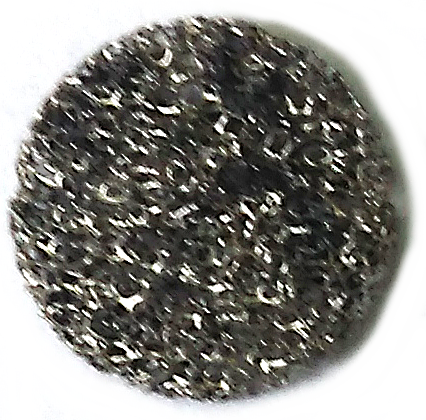
\includegraphics[width=\textwidth]{electrode_polvo_ni.png}
			\caption{\mPolvoNiquel}
			\label{fig:electrode_powder_ni}
		\end{subfigure}
		\begin{subfigure}[b]{\electrodesWidth}
			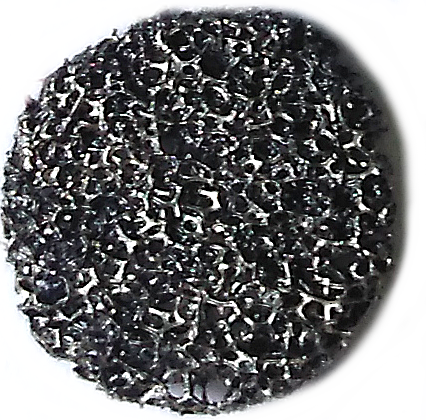
\includegraphics[width=\textwidth]{electrode_polvo_pmma_ni.png}
			\caption{\mPolvoNiquelPMMA}
			\label{fig:electrode_powder_pmma_ni}
		\end{subfigure}
	\end{adjustbox}
	\caption[Electrodos utilizados en la celda de prueba de supercondensador]{Electrodos utilizados en la celda de pruebas de supercondensador, nombrados por sus alias de la tabla \ref{tab:electrodos_construidos}. El electrodo \mLiofilizadoAcero de la figura \subref{fig:electrode_lio}, se introduce en la celda tal cual se muestra, procurando cubrir todo el sustrato de acero.}
	\label{fig:electrodes}
\end{figure}

\section{Caracterización electroquímica}
Los electrodos son sometidos a pruebas electroquímicas para estudiar su desempeño. Estas pruebas incluyen: voltametría cíclica (CV), ciclos de carga y descarga a corriente constante, espectroscopía de impedancia electroquímica (EIS). Todas las mediciones electroquímicas son hechas con un potenciostato/galvanostato Gamry (Interface 5000E). Además de los electrodos construidos con rGO, también se mide el comportamiento de los sustratos de acero y níquel.

La metodología de medición para cada muestra es la siguiente: inicialmente se mide la masa de material depositado. Luego, se limpia la celda de pruebas con etanol, para eliminar cualquier residuo de mediciones anteriores. Posteriormente se arma el supercondensador al interior de la celda, agregando una gota de electrolito al separador de papel y cerrándola con la precaución de que las juntas tóricas sellen correctamente el interior de la celda. Inmediatamente se prosigue con las mediciones electroquímicas. Primero se realizan ciclos de voltametría a diferentes velocidades de barrido: 25, 50, 100, 200, y 400 mV/s, tres ciclos para cada una, y solo se toma la última curva (esto para remover la carga acumulada en el dispositivo bajo prueba).  Luego de la voltametría cíclica, el espectro de impedancia es obtenido y se procede con los ciclos de carga y descarga a corriente constante a 1 A/g, exceptuando las muestras de polvo más pmma (polimetilmetacrilato) en disco de acero y polvo en espuma de níquel, donde la densidad de corriente se disminuyó 0,1 A/g debido a la alta resistencia en serie equivalente\footnote{La alta resistencia en serie equivalente produce una caída de potencial mayor al voltaje de trabajo entre los terminales del dispositivo, haciendo la medición irrealizable. }. Una vez finalizados, se vuelve a realizar la voltametría cíclica, para conocer el efecto que tuvo el proceso de carga y descarga en el dispositivo, finalizando las mediciones electroquímicas. Los parámetros utilizados para cada prueba se detallan en la tabla \ref{tab:elec_config}.


\begin{table}[h!]
	\centering
	\caption[Parámetros de cada medición electroquímica]{Parámetros de cada medición electroquímica.}
	\begin{tabular}{ l r }
		Voltametría cíclica &  \\
		\hline
		Voltaje inicial [V] & 0 \\
		Límite inferior [V] & -0,8 \\
		Límite superior [V] & 0,8  \\
		Número de ciclos & 3 \\
		Velocidad de barrido [mV/s] & 25, 50, 100, 200, 400 \\
		& \\
		Carga y descarga cíclica & \\
		\hline
		Densidad de corriente [A/g] & 0,1 ó 	1 \\
		Número de ciclos & 1000 \\
		Límite inferior [V] & 0 \\
		Límite superior [V] & 1 \\
		& \\
		Espectroscopía de impedancia electroqúimica & \\
		\hline
		Frecuencia inicial	&	1 MHz \\
		Frecuencia final	&	0.1 Hz \\
		Corriente de exitación & 1 mA rms \\ 
	\end{tabular}
	\label{tab:elec_config}
\end{table}

\section{Resultados y análisis}

Los resultados son presentados en una serie de gráficos para cada muestra de la tabla \ref{tab:electrodos_construidos} en el anexo \ref{sec:caracterizacion_electroquimica}. En esta sección se presentan resúmenes y comparaciones de los resultados obtenidos.

En la figura \ref{fig:resumen_cv} se comparan voltametrías a una velocidad de barrido de 100 mV/s, antes y después de 1000 ciclos de carga y descarga. De los gráficos resaltan dos curvas de mayor área, que de acuerdo a la ecuación \ref{eq:cyclic_voltametry}, esta es proporcional a la capacidad específica del supercondensador. Estas dos curvas corresponden a muestras en formato de papel y liofilizada, donde la densidad de corriente máxima es un orden de magnitud mayor al resto de las muestras, alcanzado aproximadamente 5 A/g, mientras el resto bordea los 0,5 A/g. Esto se ve reflejado al momento de calcular la capacidad específica como se muestra en la tabla \ref{tab:resumen_capacitancia}.

\begin{figure}[h!]
	\centering
	\begin{subfigure}[t!]{0.4\textwidth}
		\begin{tikzpicture}[scale=\plotscale,trim axis right,trim axis left]
		\begin{axis}
		[
		CVStyle,
		legend entries={\mPapelAcero, \mLiofilizadoAcero}
		]
		\addplot table [x=Voltaje, y expr=\thisrow{Corriente}/0.0006 ] {./Data/CV_CRGO300517_11/raw/sample3.txt};
		\addplot table [x=Voltaje, y expr=\thisrow{Corriente}/0.0006 ] {./Data/CV_CRGO300517_13/raw/sample3.txt};
		\end{axis}
		\end{tikzpicture}
		\subcaption{Antes de 1000 ciclos de carga y descarga.}
	\end{subfigure}\hfill
	\begin{subfigure}[t!]{0.4\textwidth}
		\begin{tikzpicture}[scale=\plotscale,trim axis right,trim axis left]
		\begin{axis}[
		CVStyle,
		legend entries={\mPolvoAcero, \mPolvoAceroPMMA, \mPolvoNiquel, \mPolvoNiquelPMMA},
		cycle list shift=2
		]
		\addplot table [x=Voltaje, y expr=\thisrow{Corriente}/0.0004 ] {./Data/CV_CRGO300517_9/raw/sample3.txt};
		\addplot table [x=Voltaje, y expr=\thisrow{Corriente}/0.0028 ] {./Data/CV_CRGO300517_3/raw/sample3.txt};
		\addplot table [x=Voltaje, y expr=\thisrow{Corriente}/0.0009 ] {./Data/CV_CRGO300517_5/raw/sample3.txt};
		\addplot table [x=Voltaje, y expr=\thisrow{Corriente}/0.0008 ] {./Data/CV_CRGO300517_7/raw/sample3.txt};	
		\end{axis}
		\end{tikzpicture}
		\subcaption{Antes de 1000 ciclos de carga y descarga.}
	\end{subfigure}
	\begin{subfigure}[t!]{0.4\textwidth}
		\begin{tikzpicture}[scale=\plotscale,trim axis right,trim axis left]
		\begin{axis}[
		CVStyle,
		legend entries={\mPapelAcero, \mLiofilizadoAcero}
		]
		\addplot table [x=Voltaje, y expr=\thisrow{Corriente}/0.0006 ] {./Data/CV_CRGO300517_12/raw/sample3.txt};
		\addplot table [x=Voltaje, y expr=\thisrow{Corriente}/0.0006 ] {./Data/CV_CRGO300517_14/raw/sample3.txt};	
		\end{axis}
		\end{tikzpicture}
		\subcaption{Después de 1000 ciclos de carga y descarga.}
	\end{subfigure}\hfill
	\begin{subfigure}[t!]{0.4\textwidth}
		\begin{tikzpicture}[scale=\plotscale,trim axis right,trim axis left]
		\begin{axis}[
		CVStyle,
		legend entries={\mPolvoAcero, \mPolvoAceroPMMA, \mPolvoNiquel, \mPolvoNiquelPMMA},
		cycle list shift=2
		]
		\addplot table [x=Voltaje, y expr=\thisrow{Corriente}/0.0004 ] {./Data/CV_CRGO300517_10/raw/sample3.txt};
		\addplot table [x=Voltaje, y expr=\thisrow{Corriente}/0.0028 ] {./Data/CV_CRGO300517_4/raw/sample3.txt};
		\addplot table [x=Voltaje, y expr=\thisrow{Corriente}/0.0009 ] {./Data/CV_CRGO300517_6/raw/sample3.txt};
		\addplot table [x=Voltaje, y expr=\thisrow{Corriente}/0.0008 ] {./Data/CV_CRGO300517_7/raw/sample3.txt};
		\end{axis}
		\end{tikzpicture}
		\subcaption{Después de 1000 ciclos de carga y descarga.}
	\end{subfigure}
	\caption[Resumen voltametría cíclica a 100 mV/s antes y después de 1000 ciclos de carga y descarga]{Resumen voltametría cíclica a 100 mV/s antes y después de 1000 ciclos de carga y descarga. Las muestras son separadas en dos gráficos para mejorar su visualización.}
	\label{fig:resumen_cv}
\end{figure}

\begin{table}[h!]
	\centering
	\caption{Resumen de capacitancia y capacitancia específica a 100 mV/s.}
	\begin{tabular}{ l l c c c }
		\multirow{2}{*}{Muestra}& \multirow{2}{*}{Masa [mg]}& \multirow{2}{*}{Capacitancia [mF]}	& Capacitancia & \multirow{2}{*}{Error}\\
								&         			      & 										& específica [F/g]     &			\\
		\hline
		\mSustratoAcero		&  -            &			0.1			&	-				&	-		\\
		\mPolvoAcero		& 0,4 $\pm$ 0,2 &			1.2			&	3.0	$\pm$ 1.5	&	50\%	\\
		\mPolvoAceroPMMA	& 2,8 $\pm$ 0,2 &			0.78		&	0.28 $\pm$ 0.02	&	7\%		\\
		\mPapelAcero		& 0,6 $\pm$ 0,1 &			16.8		&	28.0 $\pm$ 4.7	&	17\%	\\
		\mLiofilizadoAcero	& 0,6 $\pm$ 0,1 &			19.9		&	33.2 $\pm$ 5.5	&	17\%	\\
		\mSustratoNiquel	&    -          &			0.1			&	- 				&	-		\\
		\mPolvoNiquel		& 0,9 $\pm$ 0,2 &			0.3			&	0.35 $\pm$ 0.07	&	20\%	\\
		\mPolvoNiquelPMMA	& 0,8 $\pm$ 0,2 &			1.2			&	1.5	$\pm$ 0.4	&	27\%	\\
	\end{tabular}                                                          
	\label{tab:resumen_capacitancia}
\end{table}

En la figura \ref{fig:resumen_eis} se muestran gráficos de Nyquist obtenidos de los espectros de impedancia para distintas muestras, siguiendo el procedimiento experimental, este es tomado inmediatamente después de realizada primera voltametría cíclica. El semicírculo que se forma en alta frecuencia, da cuenta de que las muestras en formato de papel y liofilizada tienen menor resistencia en serie equivalente que el resto de las muestras \citep{Wang2009}, y el comportamiento lineal en bajas frecuencias indica un comportamiento puramente capacitivo, entre más vertical sea esta región, el supercondensador se acerca más a uno ideal \citep{Stoller2008}.

\begin{figure}[h!]
	\centering
	\begin{subfigure}[t!]{0.4\textwidth}
		\begin{tikzpicture}[scale=\plotscale,trim axis right,trim axis left]
		\begin{axis}[
		EISStyle,
		every axis legend/.append style={
			font=\tiny,
			at={(0.02,0.98)},
			anchor=north west,
		},
		legend entries = {\mPapelAcero, \mLiofilizadoAcero}
		]
		\pgfplotstableread{./Data/CV_CRGO300517_11/raw/eisgalv.txt}{\eistable};
		\pgfplotstablegetrowsof{\eistable}
		\pgfmathsetmacro{\N}{\pgfplotsretval}
		\addplot table [only marks, x=Zreal, y expr=\thisrow{Zimag}*-1] {\eistable}
		node[pos=(1-1)/(\N-1), pin=right:{1 MHz}]{}
		node[pos=(\N-1)/(\N-1), pin=left:{0,1 Hz}]{};
		\pgfplotstableread{./Data/CV_CRGO300517_13/raw/eisgalv.txt}{\eistable};
		\pgfplotstablegetrowsof{\eistable}
		\addplot table [only marks, x=Zreal, y expr=\thisrow{Zimag}*-1] {\eistable}
		node[pos=(1-1)/(\N-1), pin=right:{1 MHz}]{}
		node[pos=(40-1)/(\N-1), ]{}
		node[pos=(\N-1)/(\N-1), pin=left:{0,1 Hz}]{};
		\end{axis}
		\end{tikzpicture}
	\end{subfigure}\hfill
	\begin{subfigure}[t!]{0.4\textwidth}
		\begin{tikzpicture}[scale=\plotscale,trim axis right,trim axis left]
		\begin{axis}[
		EISStyle,
		every axis legend/.append style={
			font=\tiny,
			at={(0.98,0.02)},
			anchor=south east,
		},
		legend entries = {\mPolvoAcero, \mPolvoAceroPMMA, \mPolvoNiquel, \mPolvoNiquelPMMA},
		cycle list shift=2
		]
		\pgfplotstableread{./Data/CV_CRGO300517_9/raw/eisgalv.txt}{\eistable};
		\pgfplotstablegetrowsof{\eistable}
		\pgfmathsetmacro{\N}{\pgfplotsretval}
		\addplot table [only marks, x=Zreal, y expr=\thisrow{Zimag}*-1] {\eistable}
		node[pos=(1-1)/(\N-1), pin=right:{1 MHz}]{}
		node[pos=(\N-1)/(\N-1), pin=left:{0,1 Hz}]{};
		\pgfplotstableread{./Data/CV_CRGO300517_3/raw/eisgalv.txt}{\eistable};
		\pgfplotstablegetrowsof{\eistable}
		\addplot table [only marks, x=Zreal, y expr=\thisrow{Zimag}*-1] {\eistable}
		node[pos=(1-1)/(\N-1), pin=right:{1 MHz}]{}
		node[pos=(\N-1)/(\N-1), pin=left:{0,1 Hz}]{};
		\pgfplotstableread{./Data/CV_CRGO300517_5/raw/eisgalv.txt}{\eistable};
		\pgfplotstablegetrowsof{\eistable}
		\addplot table [only marks, x=Zreal, y expr=\thisrow{Zimag}*-1] {\eistable}
		node[pos=(1-1)/(\N-1), pin=right:{1 MHz}]{}
		node[pos=(\N-1)/(\N-1), pin=left:{0,1 Hz}]{};
		\pgfplotstableread{./Data/CV_CRGO300517_7/raw/eisgalv.txt}{\eistable};
		\pgfplotstablegetrowsof{\eistable}
		\addplot table [only marks, x=Zreal, y expr=\thisrow{Zimag}*-1] {\eistable}
		node[pos=(1-1)/(\N-1), pin=right:{1 MHz}]{}
		node[pos=(\N-1)/(\N-1), pin=left:{0,1 Hz}]{};
		\end{axis}
		\end{tikzpicture}
	\end{subfigure}
	\caption[Resumen del espectro de impedancia electroquímica]{Resumen del espectro de impedancia electroquímica. Las muestras son separadas en dos gráficos para mejorar su visualización.}
	\label{fig:resumen_eis}
\end{figure}

En la figura \ref{fig:resumen_ccd} se muestra el segundo ciclo de carga y descarga para cada muestra, pues en el primero el supercondensador comienza con una carga residual y la carga empieza	 en un voltaje arbitrario que no refleja el comportamiento del supercondensador. El tiempo que toma en completar un ciclo es proporcional a la capacidad específica del dispositivo, ya que las mediciones son hechas a 1 A/g, exceptuando la muestra de polvo en espuma de níquel, donde la densidad de corriente es de 0,1 A/g.
La muestra liofilizada en acero exhibe el mayor tiempo de carga y descarga, casi 120 segundos, casi el doble de la muestra de papel en acero y uno o dos órdenes de magnitud mayor al resto.
Otro dato útil rescatable de esta medición, es la resistencia en serie equivalente del dispositivo. Esta se traduce en una caída de potencial al comenzar la descarga, o como un offset en proceso de carga. En la tabla \ref{tab:esr} se muestra la resistencia en serie equivalente calculada a partir de los voltajes $V_1$, $V_2$ y la corriente $I$ de acuerdo a la siguiente ecuación:

\begin{equation}
	R_{S}=\frac{\left(V_2-V_1\right)}{I},
\end{equation}

donde $V_1$ es el voltaje más alto durante la carga, y $V_2$ el más alto durante la descarga.

Las muestras de papel en acero y liofilizada en acero, tienen la menor resistencia en serie equivalente, 141 y 150 [$\Omega$] respectivamente, el resto es hasta 10 veces más grande. 
\begin{figure}[h!]
	\centering
	\begin{subfigure}{0.4\textwidth}
		\begin{tikzpicture}[scale=\plotscale,trim axis right,trim axis left]
		\begin{axis}[CCDStyle,
		every axis legend/.append style={
			font=\tiny,
			at={(0.98,0.98)},
			anchor=north east,
		},
		legend entries={\mPapelAcero, \mLiofilizadoAcero}]
%		\addplot+[restrict x to domain=0:4.146667] table [ x expr=\thisrow{Time}-5.22166600000000, y expr=\thisrow{Voltage} ] {./Data/CV_CRGO300517_9/raw/chargedischarge.txt};
%		\addplot+[restrict x to domain=0:5.748327] table [ x expr=\thisrow{Time}-12.7000030000000, y expr=\thisrow{Voltage} ] {./Data/CV_CRGO300517_3/raw/chargedischarge.txt};
		\addplot+[restrict x to domain=0:62.000063] table [ x expr=\thisrow{Time}-63.3333370000000, y expr=\thisrow{Voltage} ] {./Data/CV_CRGO300517_11/raw/chargedischarge.txt};
		\addplot+[restrict x to domain=0:113.320033] table [ x expr=\thisrow{Time}-138.664967000000, y expr=\thisrow{Voltage} ] {./Data/CV_CRGO300517_13/raw/chargedischarge.txt};
%		\addplot+[restrict x to domain=0:5.743334] table [ x expr=\thisrow{Time}-5.48000000000000, y expr=\thisrow{Voltage} ] {./Data/CV_CRGO300517_5/raw/chargedischarge.txt};
%		\addplot+[restrict x to domain=0:1.088334] table [ x expr=\thisrow{Time}-2.29000000000000, y expr=\thisrow{Voltage} ] {./Data/CV_CRGO300517_7/raw/chargedischarge.txt};
		\end{axis}
		\end{tikzpicture}
	\end{subfigure}\hfill
	\begin{subfigure}{0.4\textwidth}
		\begin{tikzpicture}[scale=\plotscale,trim axis right,trim axis left]
		\begin{axis}[CCDStyle,
		every axis legend/.append style={
			font=\tiny,
			at={(0.68,0.88)},
			anchor=north west,
		},
		legend entries={\mPolvoAcero, \mPolvoAceroPMMA, \mPolvoNiquel, \mPolvoNiquelPMMA},
		cycle list shift=2
		]
		\addplot+[restrict x to domain=0:4.146667] table [ x expr=\thisrow{Time}-5.22166600000000, y expr=\thisrow{Voltage} ] {./Data/CV_CRGO300517_9/raw/chargedischarge.txt};
		\addplot+[restrict x to domain=0:5.748327] table [ x expr=\thisrow{Time}-12.7000030000000, y expr=\thisrow{Voltage} ] {./Data/CV_CRGO300517_3/raw/chargedischarge.txt};
%		\addplot+[restrict x to domain=0:62.000063] table [ x expr=\thisrow{Time}-63.3333370000000, y expr=\thisrow{Voltage} ] {./Data/CV_CRGO300517_11/raw/chargedischarge.txt};
%		\addplot+[restrict x to domain=0:113.320033] table [ x expr=\thisrow{Time}-138.664967000000, y expr=\thisrow{Voltage} ] {./Data/CV_CRGO300517_13/raw/chargedischarge.txt};
		\addplot+[restrict x to domain=0:5.743334] table [ x expr=\thisrow{Time}-5.48000000000000, y expr=\thisrow{Voltage} ] {./Data/CV_CRGO300517_5/raw/chargedischarge.txt};
		\addplot+[restrict x to domain=0:1.088334] table [ x expr=\thisrow{Time}-2.29000000000000, y expr=\thisrow{Voltage} ] {./Data/CV_CRGO300517_7/raw/chargedischarge.txt};
		\end{axis}
		\end{tikzpicture}
	\end{subfigure}
	\caption[Resumen de carga y descarga cíclica]{Resumen de carga y descarga cíclica a 1 A/g, exceptuando las muestras de polvo más pmma en disco de acero y polvo en espuma de níquel donde la densidad de corriente es de 0,1 A/g. Las muestras son separadas en dos gráficos para mejorar su visualización.}
	\label{fig:resumen_ccd}
\end{figure}


\begin{table}[h!]
	\centering
	\caption{Resistencia en serie equivalente calculada de los ciclos de carga y descarga.}
	\begin{tabular}{l c c c c}
			Muestra	&	$\mathrm{V_1}$ [mV]	&	$\mathrm{V_2}$ [mV]	&	Corriente [mA]	&	Resistencia [$\Omega$]	\\
		\hline
		\mPolvoAceroPMMA		&	1.000	&	596	&	-0,279	&	1.447	\\
		\mPolvoNiquel			&	1.000	&	854	&	-0,088	&	1.656	\\
		\mPolvoNiquelPMMA		&	999		&	402	&	-0,799	&	748		\\
		\mPolvoAcero			&	1.000	&	719	&	-0,398	&	705		\\
		\mPapelAcero			&	996		&	911	&	-0,599	&	141		\\
		\mLiofilizadoAcero		&	1.000	&	909	&	-0,599	&	150		\\
	\end{tabular}
	\label{tab:esr}
\end{table}


En la figura \ref{fig:resumen_cs} se muestra un gráfico comparativo para las capacidades específicas calculadas a partir de las curvas de voltametría. Como es de esperarse, las muestra de papel en acero y liofilizada en acero exhiben la mayor capacitancia específica para todas las velocidades de barrido, tanto antes como después de los ciclos de carga y descarga. La muestra liofilizada aumenta su capacidad específica luego de los ciclos de carga y descarga, comportamiento que no se observa en la muestra de papel en acero.




\begin{figure}[h]
	\centering
	\begin{subfigure}[t]{0.4\textwidth}
		\begin{tikzpicture}[scale=\plotscale,trim axis right,trim axis left]
			\begin{semilogxaxis}[
			SCStyle,
			only marks,
			xtick = {25, 50, 100, 200, 400},
			xticklabels = {25, 50, 100, 200, 400},
			ylabel = {Capacidad específica [F/g]},
			ymin = 0,
			ymax = 50,
			every axis legend/.append style={
				font=\tiny,
				at={(0.98,0.98)},
				anchor=north east,
			},
			legend entries={\mPapelAcero, \mLiofilizadoAcero, \mPolvoAcero, \mPolvoAceroPMMA, \mPolvoNiquel, \mPolvoNiquelPMMA},
			]
			\addplot+ [error bars/.cd, y dir=both, y fixed relative=0.16666666666] table [y expr=\thisrow{Capacitancia}] {./Data/CV_CRGO300517_11/raw/capacitance.txt};
			\addplot+ [error bars/.cd, y dir=both, y fixed relative=0.16666666666] table [y expr=\thisrow{Capacitancia}] {./Data/CV_CRGO300517_13/raw/capacitance.txt};
			\addplot+ [error bars/.cd, y dir=both, y fixed relative=0.5] table [y expr=\thisrow{Capacitancia}] {./Data/CV_CRGO300517_9/raw/capacitance.txt};
			\addplot+ [error bars/.cd, y dir=both, y fixed relative=0.07142857142] table [y expr=\thisrow{Capacitancia}] {./Data/CV_CRGO300517_3/raw/capacitance.txt};
			\addplot+ [error bars/.cd, y dir=both, y fixed relative=0.22222222222] table [y expr=\thisrow{Capacitancia}] {./Data/CV_CRGO300517_5/raw/capacitance.txt};
			\addplot+ [error bars/.cd, y dir=both, y fixed relative=0.25] table [y expr=\thisrow{Capacitancia}] {./Data/CV_CRGO300517_7/raw/capacitance.txt};
			
			\end{semilogxaxis}
		\end{tikzpicture}
		\caption{Capacidad específica antes de 1000 ciclos de carga y descarga. }
	\end{subfigure}\hfill
	\begin{subfigure}[t]{0.4\textwidth}
		\begin{tikzpicture}[scale=\plotscale,trim axis right,trim axis left]
		\begin{semilogxaxis}[
		SCStyle,
		only marks,
		xtick = {25, 50, 100, 200, 400},
		xticklabels = {25, 50, 100, 200, 400},
		ylabel = {Capacidad específica [F/g]},
		ymin = 0,
		ymax = 50,
		every axis legend/.append style={
			font=\tiny,
			at={(0.98,0.98)},
			anchor=north west,
		},
		legend entries={\mPapelAcero, \mLiofilizadoAcero, \mPolvoAcero, \mPolvoAceroPMMA, \mPolvoNiquel, \mPolvoNiquelPMMA},
		]
		\addplot+ [error bars/.cd, y dir=both, y fixed relative=0.16666666666] table [y expr=\thisrow{Capacitancia}] {./Data/CV_CRGO300517_12/raw/capacitance.txt};
		\addplot+ [error bars/.cd, y dir=both, y fixed relative=0.16666666666] table [y expr=\thisrow{Capacitancia}] {./Data/CV_CRGO300517_14/raw/capacitance.txt};
		\addplot+ [error bars/.cd, y dir=both, y fixed relative=0.50000000000] table [y expr=\thisrow{Capacitancia}] {./Data/CV_CRGO300517_10/raw/capacitance.txt};
		\addplot+ [error bars/.cd, y dir=both, y fixed relative=0.07142857142] table [y expr=\thisrow{Capacitancia}] {./Data/CV_CRGO300517_4/raw/capacitance.txt};
		\addplot+ [error bars/.cd, y dir=both, y fixed relative=0.22222222222] table [y expr=\thisrow{Capacitancia}] {./Data/CV_CRGO300517_6/raw/capacitance.txt};
		\addplot+ [error bars/.cd, y dir=both, y fixed relative=0.25000000000] table [y expr=\thisrow{Capacitancia}] {./Data/CV_CRGO300517_8/raw/capacitance.txt};
		
		\end{semilogxaxis}
		\end{tikzpicture}
		\caption{Capacidad específica después de 1000 ciclos de carga y descarga. }
	\end{subfigure}
	\caption[Resumen de la capacidad específica]{Resumen de la capacidad específica.}
	\label{fig:resumen_cs}
\end{figure}







\chapter{Conclusiones}
%\addcontentsline{toc}{chapter}{Conclusiones}
En este trabajo de tesis se implementó un método efectivo para medir el desempeño de materiales basados en carbono como electrodos de supercondensadores, que resultó ser apropiado para determinar diferencias en la construcción de los electrodos. Además, se sintetizó un material de carbono para ser utilizado como electrodo en dichos condensadores.

Comparando la capacidad específica medida para los electrodos de polvo en sustrato de acero (\mPolvoAcero), y el de polvo en espuma de níquel (\mPolvoNiquel), se observa que el sustrato de acero se desempeña mejor que el de níquel, a pesar de que el sustrato de níquel posee mayor area superficial.

El gráfico de Nyquist revela que los electrodos que exhiben un comportamiento más cercano al esperado para un supercondensador, son las 
muestras de papel y liofilizado.

\chapter*{Anexo}
\addcontentsline{toc}{chapter}{Anexo}

\SCGraphsNoMass{CV_Steel_Disk_No_Material_1}{CV_Steel_Disk_No_Material_2}{0}{16}{1954.91833300000}{Disco de acero sin material.}{200}
\SCGraphs{CV_CRGO300517_9}{CV_CRGO300517_10}{0.0004}{10}{3101.89233300000}{Polvo en disco de acero. Masa = 0.4 mg.}{0.0002}
\SCGraphs{CV_CRGO300517_3}{CV_CRGO300517_4}{0.0028}{20}{2105.33533300000}{Polvo + PMMA en disco de acero. Masa = 2.8 mg.}{0.0002}
\SCGraphs{CV_CRGO300517_11}{CV_CRGO300517_12}{0.0006}{250}{45656.2866670000}{Papel en disco de acero. Masa = 0.6 mg.}{0.0001}
\SCGraphs{CV_CRGO300517_13}{CV_CRGO300517_14}{0.0006}{465}{86333.0367000000}{Material liofilizado en disco de acero. Masa = 0.6 mg.}{0.0001}

\SCGraphsNoMass{CV_Nickel_Foam_No_Material_1}{CV_Nickel_Foam_No_Material_2}{0}{12}{2399.28233300000}{Espuma de níquel sin material.}{200}
\SCGraphs{CV_CRGO300517_5}{CV_CRGO300517_6}{0.0009}{12}{4328.46733300000}{Polvo en espuma de níquel. Masa = 0.9 mg.}{0.0002}
\SCGraphs{CV_CRGO300517_7}{CV_CRGO300517_8}{0.0008}{5}{771.593133000000}{Polvo + PMMA en espuma de níquel. Masa = 0.8 mg.}{0.0002}

%%ÍNDICE ANALÍTICO
\newpage
\printindex
\addcontentsline{toc}{chapter}{Índice Analítico}

%%BIBLIOGRAFÍA
\newpage
\printbibliography

\end{document}